\documentclass[english,svgnames,notes=hide,14pt]{beamer}
\usepackage{macros-ohp}

%\def\presentationtitle{Study and Application of Concept-Extraction \\ Algorithms in Statistical and \\ Programming Sciences}

\def\presentationtitle{Study and Application of Concept-Extraction \\ Algorithms in Natural Language Processing (NLP)}


\title{\large\presentationtitle}
\author{Ana-Maria Vintila\\
		\small Supervised by Professor Brenda Vo\\
		\small University of New England, Australia
	}

%Please make sure the tex is compiled twice to have all the images displayed correctly.

%Fill the date or leave it blank to not display it
\date{}

\begin{document}
\thispagestyle{empty}
%\begin{frame}[plain] %put [plain] at the end to get rid of the page number on this page
\begin{frame}
  \titlepage
  
\end{frame}



% Line spacing
\linespread{1.0}
% Change font size:
\ContentFontSize




\begin{frame}{About Me}

\begin{itemizeSpaced}{10pt}
    \pinkbox Name: Ana-Maria Vintila,  Age: 22
    \pinkbox International citizen, lived and studied in Canada for a majority of my life before returning to native Europe. 
    %\item Diligent, thrive in well-defined, scientific domains. 
    
    \item Interests: Calculus, Scala / Haskell functional programming, Probability (with Wolfram-Mathematica in ProbOnto-style)
    
    \pinkbox Currently working towards doing Master By Research in NLP and / or Finance using applied maths and Bayesian statistics. 
    
    \pinkbox Envisioning: NLP business to study text for global clients, and for financial analysis for currency exchange markets. 
    
\end{itemizeSpaced}

    
\end{frame}


\section{Introduction: Motivation for Text Processing}


\begin{frame}{Introduction: Motivation for Text Processing} %\vspace{40pt}



\begin{itemizeSpaced}{7pt}

    \item Vast amounts of knowledge are trapped in presentation media such as videos, html, pdfs, and paper as opposed to being concept-mapped, interlinked, addressable and reusable at fine grained levels. This defeats knowledge exchanges between humans and between human cognition and AI-based systems.
    
    \item It is known that concept mapping enhances human cognition. Especially in domain-specific areas of knowledge, better interlinking would be achieved if concepts would be extracted using surrounding context, accounting for polysemy and key phrases. “You shall know a word by the company it keeps” (Firth, 1957).
    
    
    \item Previous count-based models like GloVe and Word2Vec motivated recent models like models like Transformer, ELMo, BERT, Transformer-XL, XLNet, and ERNIE 2.0 to move beyond simple co-occurrence counts to extract meaning. 
    
    \item ERNIE 2.0 instead “broadens the vision to include more lexical, syntactic and semantic information from training corpora in form of named entities (like person names, location names, and organization names), semantic closeness (proximity of sentences), sentence order or discourse relations” (Sun et al., 2019). 
    
    \item \textbf{Example:} ERNIE 1.0 can associate entire entity names with other terms in a given sentence, while on the same data, BERT lacks this ability.
    
    
\end{itemizeSpaced}
\end{frame}







\begin{frame}{Aim of this Project}

To understand how good language representations are created using lexical and semantic structure, at the \emph{entity and phrase level}, using two approaches:
    
\vspace{15pt}

\begin{itemizeSpaced}{15pt}
    \item \textbf{``Study"} to inventory, compare various architectures and how they leverage entities, polysemy, context for concept extraction. 
    
    \item \textbf{``Application"} using PyTorch to illustrate a key model architecture as it is applied to machine translation (MT) task. 
\end{itemizeSpaced}
    
\end{frame}


\begin{frame}{}
    \centering \large \textbf{Word Embeddings}
\end{frame}


\begin{frame}{}
    
    \begin{definitionBlock}{Definition: Word Embedding (Words as Vectors)}
        Word embeddings are unsupervised models that capture semantic and syntactic information about words in a compact low-dimensional vector representation $\Rightarrow$ useful for reasoning about word usage and meaning (Melamud et al. 2016, p. 1).
    \end{definitionBlock}
    \vspace{-5pt}
    
    
    \begin{itemizeSpaced}{3pt}
        
        
        \pinkbox Sentence embeddings, phrase embeddings, character embeddings (for morphology)
        
        \pinkbox Can capture \textbf{vector space semantics}: can express word analogy ``man is to woman as king is to queen" with arithmetic on learned word vectors: $vector(man) - vector(woman) = vector(king) - vector(queen)$
        
    \end{itemizeSpaced}
    
    \begin{figure}[h]
    \vspace{-10pt}
    \centering
    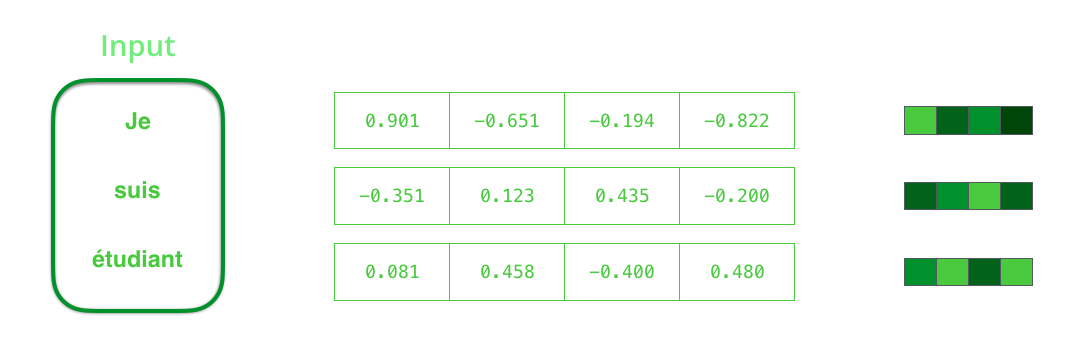
\includegraphics[width=0.8\textwidth]{imgs/example_word_embedding.png}
    \vspace{-5pt}
    \caption{\tiny \linespread{0.1} Example Word Embeddings. From \emph{Visualizing Neural Machine Translation Mechanics of Seq2Seq Models with Attention}, by Jay Alammar, 2018. \url{http://jalammar.github.io/visualizing-neural-machine-translation-mechanics-of-seq2seq-models-with-attention/}}
    \vspace{-10pt}
    \label{fig:exampleWordEmb}
    \end{figure}
    
\end{frame}



% \begin{frame}{} %{ \normalsize {\vfill\vfill Mathematically: \\How Models Make Embeddings}}
% 
%   \small\textbf{Mathematically: How Models Make Embeddings ..}
% 
% \begin{itemizeSpaced}{10pt}
%       \small
%     
%     \item a word’s conditional probability combines its \emph{embedding} and \emph{context vectors} of surrounding words, with different methods combining them differently. 
%     
%     \item Then, embeddings are fitted to text by maximizing the conditional probabilities of observed text.
%     
% \end{itemizeSpaced}
%     
% \end{frame}




\begin{frame}{What is Polysemy?}
      \small 
    
    \begin{definitionBlock}{Definition: Polysemy}
    \alert{\textbf{Polysemy}} means a word has multiple senses. 
    \end{definitionBlock}
    
    
    \begin{definitionBlock}{Definition: Distributional Hypothesis}
    \alert{\textbf{Distributional hypothesis}} is a key idea in NLP that says meaning depends on context, and words in same contexts have similar meaning (Wiedemann et al., 2019). 
    \end{definitionBlock}
\end{frame}





\begin{frame}{Static vs. Contextual Embeddings}

    \vspace{20pt}

    \begin{definitionBlock}{\footnotesize Definition: Static Embeddings}
           \alert{\textbf{Static embeddings}} (classic word vectors) assign one vector to each word, regardless of polysemy (Ethayarajh, 2019). \newline 
           
           Skip-Gram and Glove produce these ``context-free" representations because they use co-occurrence counts, not the more dynamic \textbf{language modeling} approach (Batista, 2018). 
           
    \end{definitionBlock}
    
    
    \vspace{-2pt}
    
    \begin{alertBlock}{\footnotesize Alert}
        All senses of a polysemic word are \emph{\alert{collapsed}} within a single vector representation (Ethayarajh, 2019). Confusion!  \newline 
        
        ``Plant”'s embedding would be the ``average of its different contextual semantics relating to biology, placement, manufacturing, and power generation” (Neelakantan et al., 2015).

    
    \end{alertBlock}
    
    \vspace{-2pt}
    
    \begin{definitionBlock}{\footnotesize Better: Contextual Word Embedding}
   
    A \textbf{\alert{contextual word embedding (CWE)}} captures forward and backward context using a bidirectional language model (biLM) (Antonio, 2019).   
    
    Static word embeddings are like ``look-up tables" but contextual embeddings have word type information (Smith, 2019). 
\end{definitionBlock}
      
    
\end{frame}


% 
% 
% \begin{frame}{Better: Contextual Embeddings (CWE)}
% 
% 
% \begin{definitionBlock}{Definition: Contextual Word Embedding}
%       \small
%     A \textbf{\alert{contextual word embedding (CWE)}} captures context using forward and backward history, using a bidirectional language model (biLM) (Antonio, 2019).   
%     
%     Static word embeddings are like ``look-up tables" but contextual embeddings have word type information (Smith, 2019). 
% \end{definitionBlock}
% 
% 
% \begin{itemizeSpaced}{7pt}
% 
%     \pinkbox Abandons the idea of using a fixed word sense inventory (to model polysemy) to make a vector representation for each \textbf{word type} in the vocabulary and each \textbf{word token} in a context. 
%     
%     \pinkbox Experimentally superior to static embeddings.
%     
%     \item ``sentence or context-level semantics together with word-level semantics proved to be a powerful innovation” in the NLP world (Wiedemann et al., 2019).
%     
%     
% \end{itemizeSpaced}
%     
% \end{frame}

\section{Language Models}



% ERASE ALL ?

\begin{frame}{Language Models}
    
    \begin{definitionBlock}{Definition}
    A \alert{\textbf{language model}} takes a sequence of word vectors and outputs a sequence of predicted word vectors by learning a probability distribution over words in a vocabulary.
    
    They predict words sequentially, unidirectionally, one token at a time, using some context words. 
    
    Formally, they compute the conditional probability of a word $w_t$ given a context, such as its previous $n-1$ words, where the probability is: $P(w_t | w_{t-1}, ..., w_{t-n+1})$
    
    \end{definitionBlock}
    
    
\end{frame}





% ERASE: 
\begin{frame}{Types of Language Models}
    

\begin{itemizeSpaced}{5pt}
    \item \textbf{$n$-gram language model: } an $n$-gram is a sequence of $n$ words. The model finds a word's probability based on frequencies of its constituent $n$-grams, taking just preceding $n-1$ words as context instead of the entire corpus. 
    
    \item \textbf{neural network model: } uses a linear $W \cdot x + b$ function called a neuron. By applying a nonlinear function $f(\cdot)$ to this equation and by incorporating many hidden layers and by stacking neurons together, a neural network can model any function.
    
    Has \textbf{embedding layer}, \textbf{intermediate layers} to transform embeddings, and \textbf{final layer}, which often uses softmax function to normalize word embedding matrix to create probability distribution over words. 
    
    \item \textbf{bidirectional language model (biLM): } calculates probability of a token given its \emph{forward} and \emph{backward} tokens. Uses \textbf{forward} and \textbf{backward language model}s, respectively. 
    
    
    

    \begin{figure}[h]
    \vspace{-5pt}
    \centering
    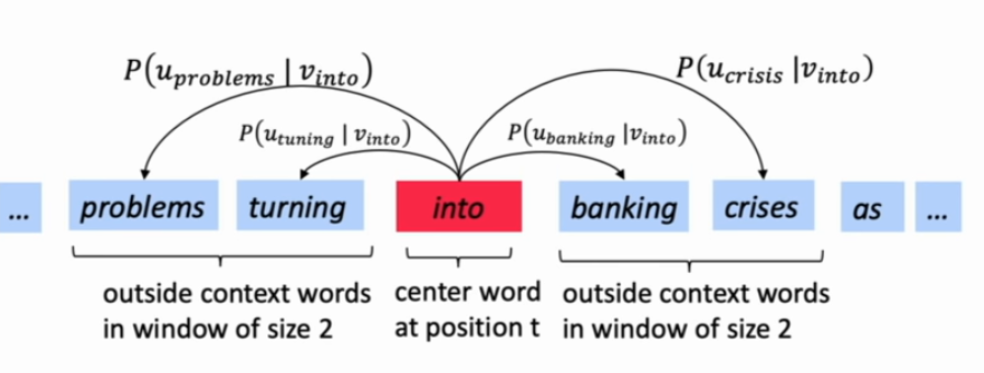
\includegraphics[width=0.65\textwidth]{imgs/bidirectional_languagemodel_banking.png}
    \vspace{-10pt}
    \caption{\tiny Example Bidirectional Language Model. From \emph{Word2Vec Overview With Vectors}, by CS224n: Natural Language Processing with Deep Learning (Stanford), 2018. \url{https://sangminwoo.github.io/2019-08-28-cs224n-lec1/}. Copyright n.d. by n.d.}
    \vspace{-5pt}
    \label{fig:bidirectionalLM}
    \end{figure}
    
\end{itemizeSpaced}

\end{frame}





% ERASE
\begin{frame}{Example: Bidirectional Language Model}


{\large \textbf{Consider the two sentences ...}


\textit{``Mary accessed the bank account.”} 

\textit{``The swan waded to the bank of the river.”}

}

\begin{alertBlock}{Warning}
    \large 
    A unidirectional contextual model would represent the target word “bank” based on `I accessed the’ but not `account.’ 
    
    Cannot capture \textbf{polysemy} of `bank’ !
\end{alertBlock}



{\large But a bidirectional language model represents ``bank” using both previous and next context to ameliorate this problem.}
    
\end{frame}

\begin{frame}{}
    \begin{center}
        \large \textbf{Word2Vec}
    \end{center}
    \vspace{20pt}
    
    \textbf{Author(s):}
    \begin{itemizeSpaced}{5pt}
    {\color{DimGrey} 
        \item Mikolov et al. (2013a) in \emph{Distributed Representations of Words and Phrases and their Compositionality}
        
        \item Mikolov et al. (2013b) in \emph{Efficient Estimation of Word Representations in Vector Space}
    }
    \end{itemizeSpaced}
\end{frame}

% -------------------------------------------------



\begin{frame}{Word2Vec: One-Hot Encodings}

    \begin{definitionBlock}{Definition: One-Hot Encoding}
    A \textbf{\alert{one-hot vector encoding}} is the simplest type of word embedding where each cell in the vector corresponds to a distinct vocabulary word. \newline 
    
    %Its dimension equals the vocabulary size.
    
    A $1$ is placed in the cell marking the position of the word in the vocabulary, and a $0$ is placed in all other cells.
    \end{definitionBlock}
    
    \begin{alertBlock}{Warning!}
    
    One-hot encodings cause ...
    
    \begin{itemize}
        \item high-dimensionality vector representations for large vocabularies, $\Rightarrow$ increased computational costs.
        
        \item similarity between (word) categories cannot be represented.
    \end{itemize} 
    
    \end{alertBlock}
    
\end{frame}



% ERASE
% \begin{frame}{Word2Vec: Basic Structure of Skip-Gram and CBOW}
%     
%     \begin{itemizeSpaced}{5pt}
%         \pinkbox Both are neural networks with one hidden layer that is a word embedding with dimension $N$. (Thus even though the vocabulary size is $V$, the goal is to learn embeddings with size $N$).
%         
%         \item input vector is $\overrightarrow{x} = (x_1,..., x_V)$ 
%         
%         \item output vector is $\overrightarrow{y} = (y_1,...,y_V)$ 
%         
%         \begin{itemize}
%             \item both are one-hot encodings
%         \end{itemize}
%         
%         \item At time $t$, they predict one output word $w_{t+j}$ (whose vector representation is $\overrightarrow{y}$), given one input word $w_t$ (whose vector representation is $\overrightarrow{x}$).
%         
%         
%         \item \textbf{Skip-Gram: }$w_{t+j}$ is the \emph{predicted context word} and $w_t$ is the \emph{input target word},
%         
%         \item \textbf{CBOW: } $w_{t+j}$ is the \emph{predicted target word} and $w_t$ is the \emph{input context word}.
%         
%         
%         \item Notation details below\footnotemark
%     
%     \end{itemizeSpaced}
% 
% \footnotetext[1]{Vectors $v_w$ and $v'_w$ are two representations of word $w$. Vector $v_w$ comes from the rows of the \textit{input layer $\rightarrow$ hidden layer weight matrix} $W$, and vector $v'_w$ comes from the rows of the \textit{hidden layer $\rightarrow$ output layer weight matrix} $W'$. We call $v_w$ the \textbf{input vector} and $v'_w$ is the \textbf{output vector} of the word $w$. }
%     
% \end{frame}



\begin{frame}{Word2Vec: Skip-Gram}\label{SkipGram}
    
    \begin{itemizeSpaced}{2pt}
        \pinkbox  \textbf{Predicts context words given a single target word: } Uses a fixed sliding window $c$, or size of the training context, around a target word, to capture context (bidirectionally) along a sentence. 
        
        \item Target center word (one-hot encoding) is input to a neural network which updates the vector with values near $1$ in cells corresponding to predicted context words.
        
    \end{itemizeSpaced}
    
    
    \begin{figure}[h]
    \vspace{-25pt}
    \centering
    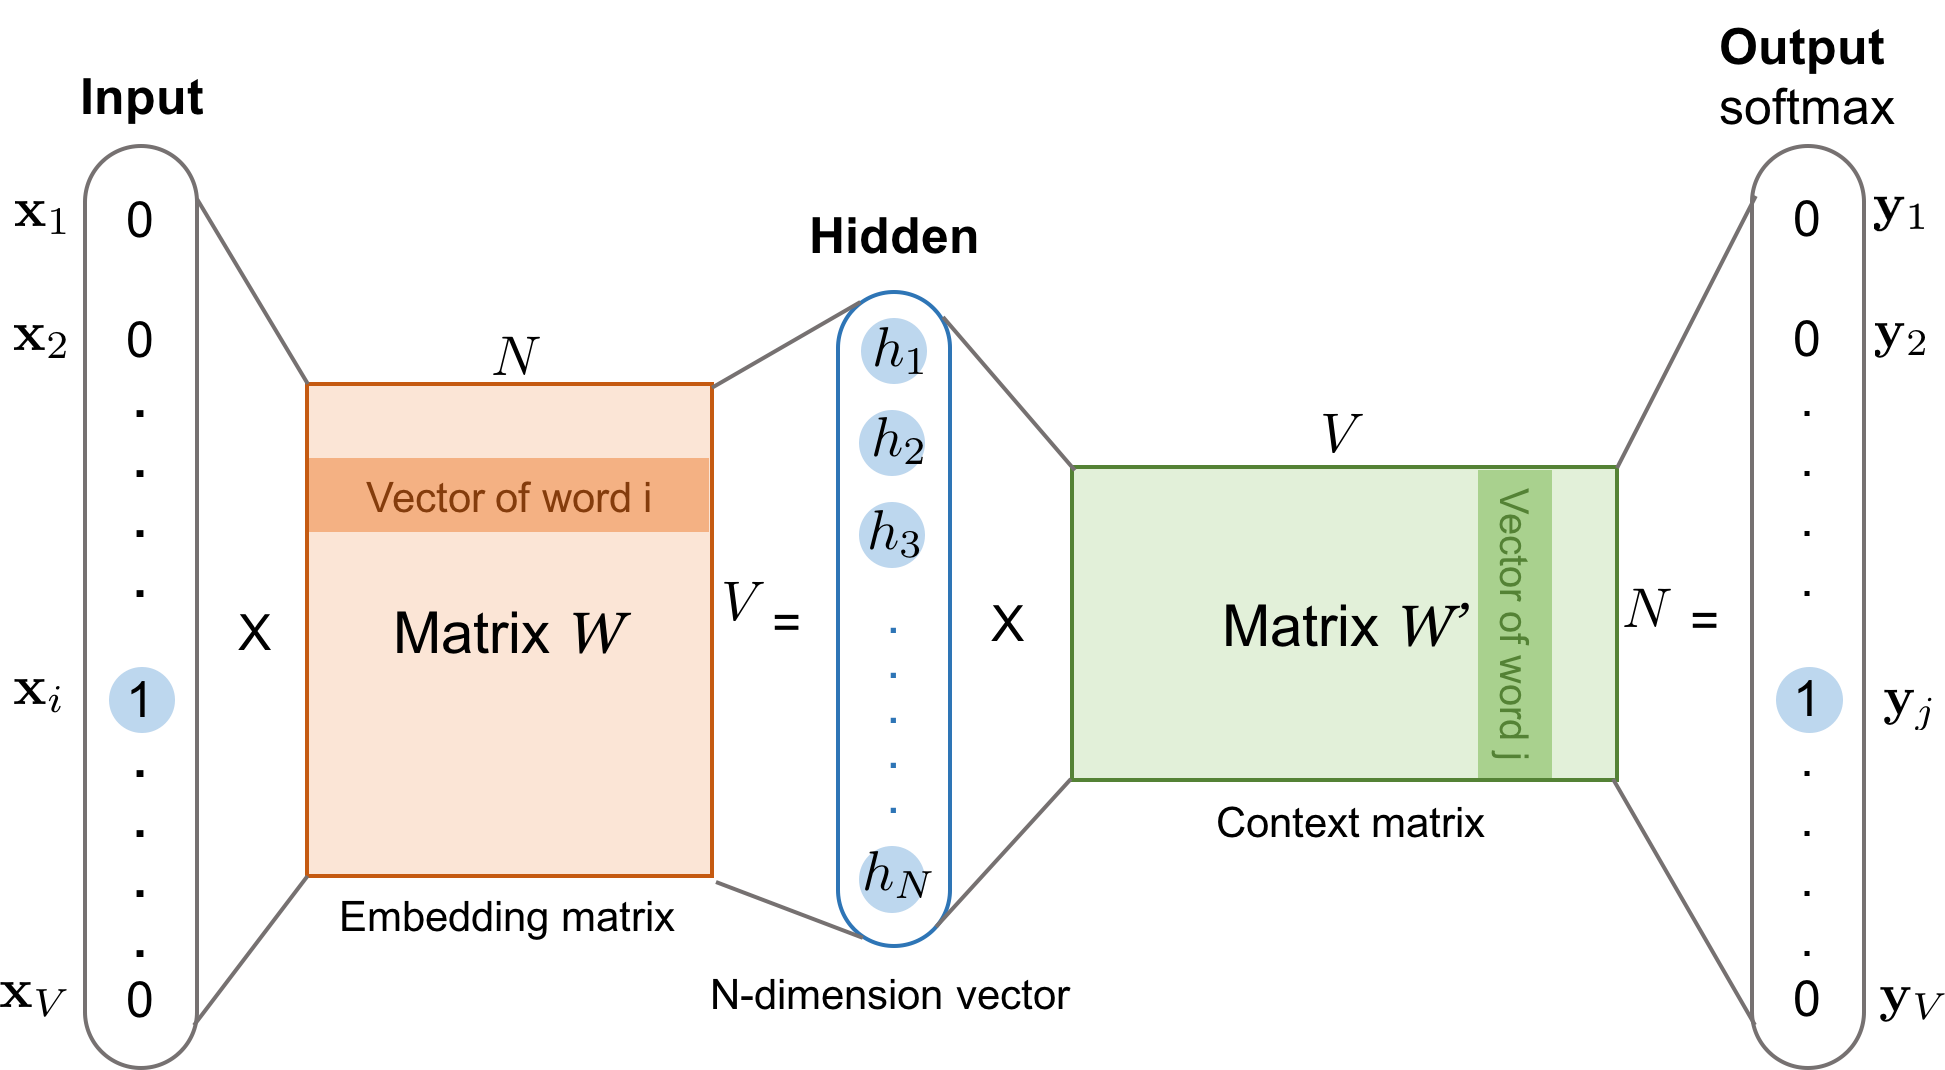
\includegraphics[width=0.7\textwidth]{imgs/skipgram_image.png}
    \vspace{-5pt}
    \caption{\tiny Skip-Gram Model; simplified version, with one input target word and one output context word. From \emph{Learning Word Embeddings}, by Lilian Weng, 2017. \url{https://lilianweng.github.io/lil-log/2017/10/15/learning-word-embedding.html}. Copyright n.d. by n.d.}
    \label{fig:SkipGram}
    \vspace{-25pt}
    \end{figure}
    
\end{frame}


\begin{frame}{Word2Vec: Continuous-Bag-of-Words (CBOW)}\label{frame:CBOW}

    \vfill 
    
    \begin{itemizeSpaced}{0pt}
        \pinkbox \textbf{Continuous bag of words model (CBOW)} is opposite of the Skip-Gram: predicts \emph{target} word based on a \emph{context} word. 
        
        \item Averages $n$ context words around target word $w_t$ to predict target (in hidden layer calculation): %\footnotemark 
        $
        \overrightarrow{h} 
        = \frac{1}{c} W \cdot \Big(\overrightarrow{x_1} + \overrightarrow{x_2} + ... + \overrightarrow{x_c} \Big) 
        = \frac{1}{c} \cdot \Big(\overrightarrow{v_{w_1}} + \overrightarrow{v_{w_2}} + ... + \overrightarrow{v_{w_c}} \Big)
        $
        
    \end{itemizeSpaced}
    
    \begin{figure}[h] 
    \vspace{-25pt}
    \centering
    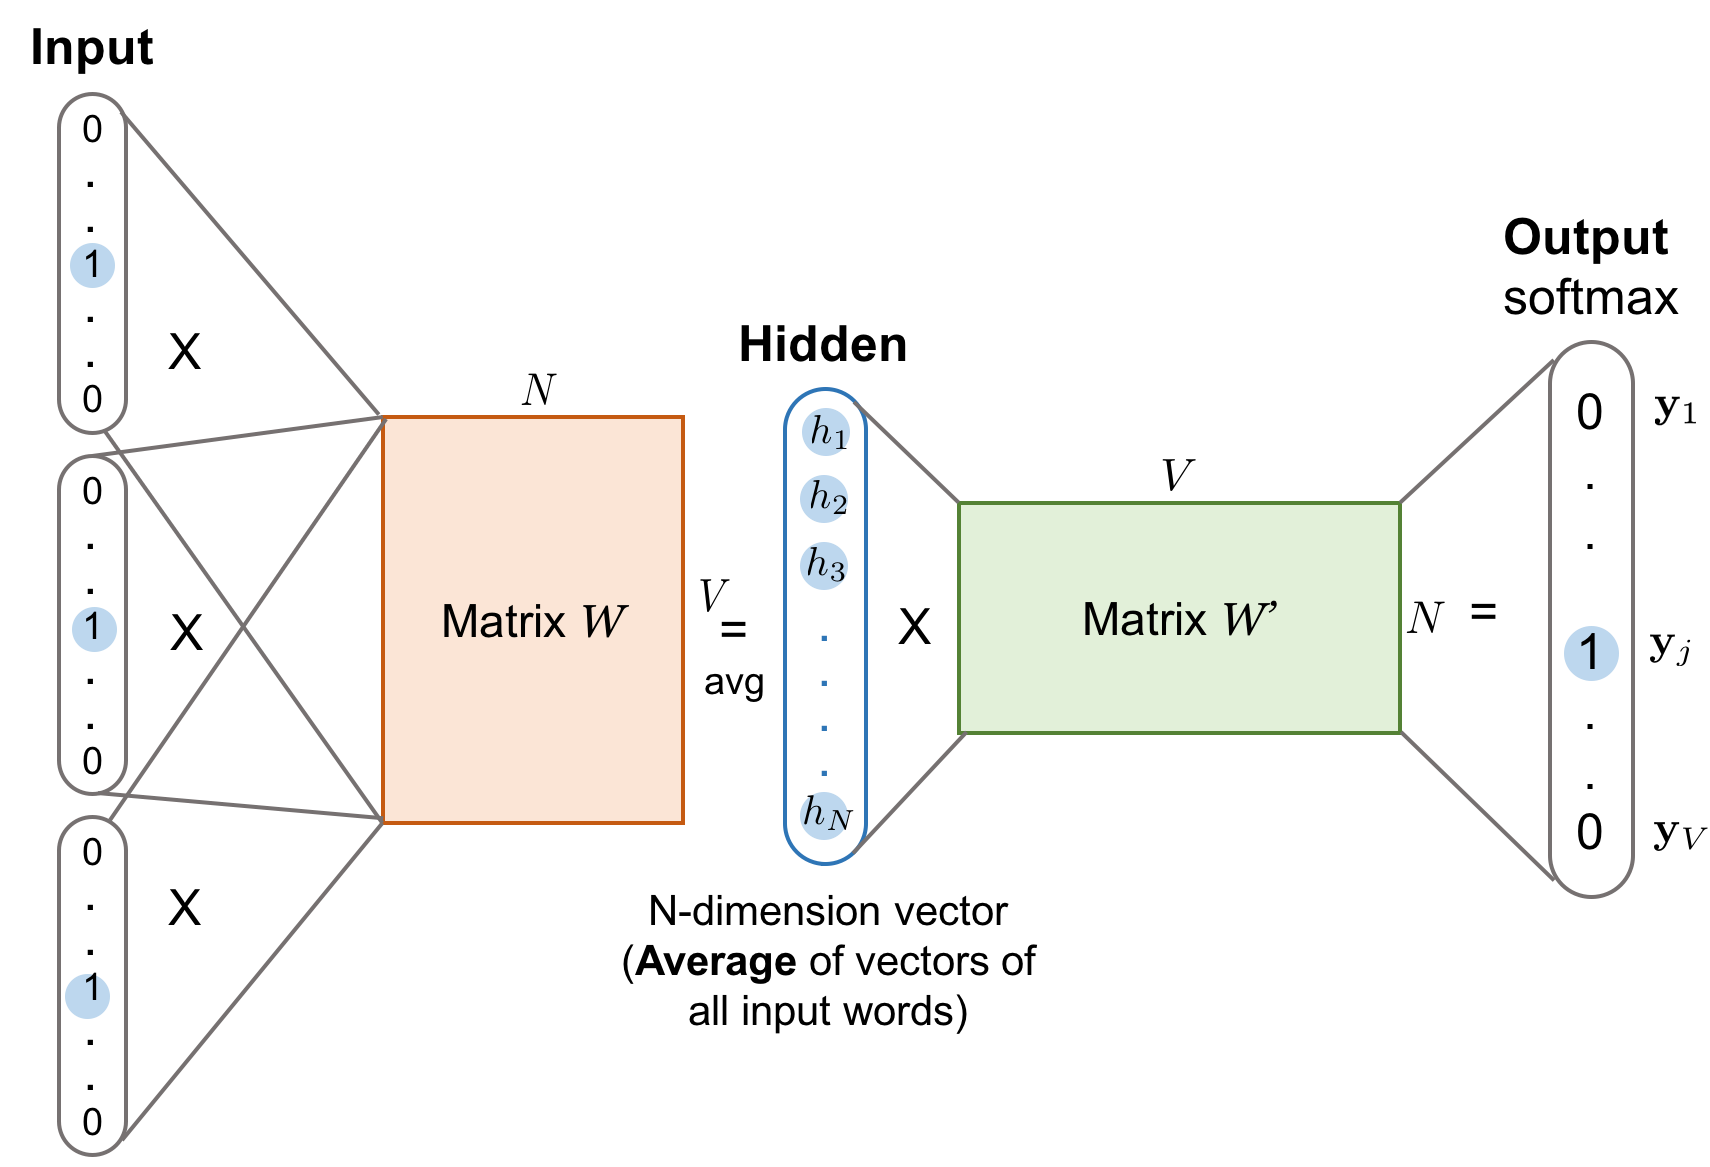
\includegraphics[width=0.6\textwidth]{imgs/cbow.png}
    \vspace{-5pt}
    \caption{\tiny CBOW Model with several one-hot encoded context words at the input layer and one target word at the output layer. From \emph{Learning Word Embeddings}, by Lilian Weng, 2017. \url{https://lilianweng.github.io/lil-log/2017/10/15/learning-word-embedding.html}}
    \label{fig:CBOW}
    \vspace{-15pt}
    \end{figure}
    
    %\footnotemark[1]{\footnotesize CBOW averaging distributional information of the context vectors makes it better suited for small datasets (Weng, 2018).}
    
\end{frame}



\begin{frame}{Phrase-Learning in Skip-Gram}
    \vfill
    
    \begin{itemizeSpaced}{2pt}
    
        \pinkbox \textbf{Problem with previous word vectors:} no \emph{phrase representation}
        
        \begin{itemizeSpaced}{2pt}
            \arrowitem “Canada” and “Air” in a phrase could not be recognized as part of a larger concept and thus combined into “Air Canada” (Mikolov et al., 2013a).
        \end{itemizeSpaced}
        
        \pinkbox \textbf{Phrase-Skip-Gram Model}: uses \emph{unigram and bigram counts} to make phrases.
        \begin{itemizeSpaced}{2pt}
            
            \item ${\large S_{phrase} = \frac{C(w_i w_j) - \delta} {C(w_i)C(w_j)} }$ where $C(\cdot)$ = count of a unigram $w_i$ or bigram $w_i w_j$ and $\delta$ is a discounting threshold to avoid making infrequent words and phrases.
            
            \item Large $S_{phrase}$ indicates the \emph{phrase} is a phrase, less likely a bigram. 
        \end{itemizeSpaced}
        
        
        \item \textbf{Result: } linear structure \textbf{additive compositionality} of word vectors 
        
        \begin{itemizeSpaced}{2pt}
            \pinkbox \textbf{Additive Compositionality: }lets some individual words be combined into a phrase and be viewed as a unique \emph{entity}, while a bigram like “this is” should remain unchanged (Mikolov et al., 2013a, p. 5).
            
            \item \textbf{How Does It Happen? } product of distributions in loss function acts like an ``and" function
        \end{itemizeSpaced} 
        
        \begin{exampleBlock}{Example: Additive Compositionality}
        
        If the phrase ``Volga River" appears numerously with ``Russian" and ``river" then: $vector(\texttt{"Russian"}) \! + \! vector(\texttt{"river"}) \; \Rightarrow \; vector(\texttt{"Volga River"})$
        
        \end{exampleBlock}
        
        
    \end{itemizeSpaced}
    
\end{frame}



\section{GloVe (Global Vectors for Word Representation)}


\begin{frame}{Problem With Word2Vec}
    
    \begin{itemizeSpaced}{0pt}
        \item \textbf{Problem: } Word2Vec uses local not global counts.  
        \begin{itemizeSpaced}{0pt}
            \item \textbf{Example: }``the" and ``cat" may occur frequently but Word2Vec does not know if this is because ``the" is a common word or because ``the" and ``cat" are actually correlated  (Kurita, 2018). 
            
        \end{itemizeSpaced}
        
        \item \textbf{Reason: } 
        \begin{itemizeSpaced}{0pt}
            \item Word2Vec implicitly optimizes over a co-occurrence matrix while streaming over input sentences $\Rightarrow$ context words are processed equally.
            
            \item Word2Vec's loss function $J = - \sum_i X_i \sum_j P_{ij} \text{log}(Q_{ij}) $ is the cross entropy between the \emph{predicted} and \emph{actual word distributions} in the context of word $i$.  \footnotemark 
            
            \item GloVe's authors say cross entropy models long-tailed distributions poorly, and here $X_i$ means equal-weighting over words. 
            
            \item Kurita (2018a) says there is no inherent justification for equal-streaming over words: GloVe uses \emph{unnormalized} probabilities. 
            
        \end{itemizeSpaced}
        
    \end{itemizeSpaced}
    
    \footnotetext[3]{\footnotesize $X_i = \sum_k X_{ik}$ is the total number of words appearing in the context of word $i$ \newline $Q_{ij} = \text{softmax} \Big( w_i \cdot w_j \Big)$ is the probability that word $j$ appears in context of word $i$}
\end{frame}




\begin{frame}{GloVe}

\begin{itemizeSpaced}{0pt}
    \item \textbf{Assumption: } words co-occur when they appear within a fixed sliding window $\Rightarrow$ reveals corpus-wide, not sentence-level word meaning.
\end{itemizeSpaced}

\begin{exampleBlock}{How GloVe Uses Co-Occurrence Ratios \footnotemark}
Consider two words $w_i =$ ``ice" and $w_j = $ ``steam". 

\begin{itemizeSpaced}{0pt}
    \item \textbf{Case 1:} For context words $\Tilde{w}_k$ related to ``ice" but not ``steam" ($\Tilde{w}_k = $ ``solid") $\Rightarrow$ expect co-occurrence probability $p_{\text{co}} \Big( \Tilde{w}_k \; | \; w_i \Big)$ is much larger than $p_{\text{co}} \Big( \Tilde{w}_k \; | \; w_j \Big)  \;\; \Rightarrow \;\; $ ratio $\frac {p_{\text{co}} \Big( \Tilde{w}_k \; | \; w_i \Big)} {p_{\text{co}} \Big( \Tilde{w}_k \; | \; w_j \Big)}$ gets very large.

    \item \textbf{Case 2: } Conversely, for words related to ``steam" but not ``ice" ($\Tilde{w}_k = $ ``gas") $\Rightarrow$ the co-occurrence ratio $\frac {p_{\text{co}} \Big( \Tilde{w}_k \; | \; w_i \Big)} {p_{\text{co}} \Big( \Tilde{w}_k \; | \; w_j \Big)}$ should be small. 

    \item \textbf{Case 3:} For $\Tilde{w}_k = $ ``water" related to both, or $\Tilde{w}_k = $ ``fashion" unrelated to either ``ice" or ``steam", then ratio $\frac {p_{\text{co}} \Big( \Tilde{w}_k \; | \; w_i \Big)} {p_{\text{co}} \Big( \Tilde{w}_k \; | \; w_j \Big)}$ is near one. 
\end{itemizeSpaced}
\end{exampleBlock}



\footnotetext[4]{GloVe defines word co-occurrence probability as: 
    $p_{\text{co}} \Big(w_k \; | \; w_i \Big) = \frac{C(w_i, w_k)}{C(w_i)}$  where $C(w_i, w_k)$ counts the co-occurrence between words $w_i$ and $w_k$.  }

\end{frame}



\begin{frame}{Performance: GloVe vs. Word2Vec}
    
    \cref{fig:gloveVsWord2vec} shows GloVe's learned embeddings have higher prediction accuracy over those of Skip-Gram and CBOW on \textbf{word analogy} and \textbf{named entity recognition (NER)}.
    
    \begin{figure}[h]
    \vspace{-5pt}
    \centering
    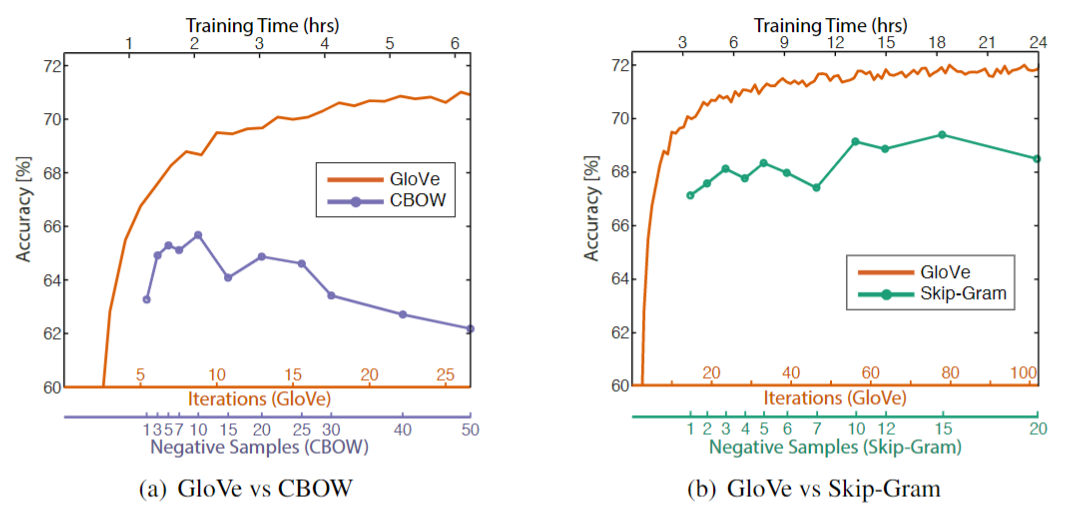
\includegraphics[width=0.99\textwidth]{imgs/table_gloveVSword2vec.png}
    \vspace{-5pt}
    \caption{\tiny Overall accuracy on word analogy task as a function of training time, which is governed by the number of iterations for GloVe and by the number of  negative samples for CBOW (a) and Skip-Gram (b). Pennington et al. (2014) train 300-dimensional vectors on the same 6B token corpus from Wikipedia and use a symmetric context window of size 10. From \emph{GloVe: Global Vectors for Word Representation}, by Pennington et al., 2014. \url{https://nlp.stanford.edu/pubs/glove.pdf}. Copyright 2014 by Pennington et al.}
    \vspace{-5pt}
    \label{fig:gloveVsWord2vec}
    \end{figure}
\end{frame}


\section{Sequence-To-Sequence Model}


\begin{frame}{Seq-To-Seq Model (Brief Overview)}
    
    \normalsize 
    {\linespread{0.3}
    
    \begin{itemizeSpaced}{7pt}
        \pinkbox Used for machine translation task. \textbf{Encoder} takes in sequence of tokens (words, phrases), processes inputs into a \emph{fixed-length} \textbf{context vector}, and sends it to \textbf{Decoder} that outputs another sequence of tokens. 
        
        \item Encoder, Decoder are often RNN's \footnotemark like LSTMs\footnotemark and GRUs\footnotemark. 
        
        \pinkbox {\color{Crimson} \textbf{Problem: }} compressing inputs into \textbf{fixed-length vector} causes \textbf{long-term dependency problem} (memory loss) since only the \emph{last hidden Encoder state is used}. 
        
        \pinkbox {\color{ForestGreen} \textbf{Solution: }}to use \textbf{attention mechanism} for selectively focusing on parts of the inputs as required (creates a context vector for \emph{each time step or word}, so all Encoder's output hidden states are used in Decoder)
        
        
    \end{itemizeSpaced} }
    
    \footnotetext[5]{\footnotesize RNN stands for \textbf{recurrent neural network}, which has a looping mechanism to share hidden states. Suffers from \textbf{long-term dependency problem}}
    
    \footnotetext[6]{\footnotesize LSTM means \textbf{long-short term memory network}, and uses forget gates to regulate memory and information flow}
    
    \footnotetext[7]{\footnotesize GRU means \textbf{gated-recurrent network}, and is a condensed version of LSTM. }
    
\end{frame}

\begin{frame}{}
    \begin{center}
        \large \textbf{Transformer}
    \end{center}
    \vspace{20pt}
    
    \textbf{Author(s):}
    \begin{itemizeSpaced}{5pt}
    {\color{DimGrey} 
        \item Vaswani et al. (2017) in \emph{Attention is All You Need}
        
    }
    \end{itemizeSpaced}
\end{frame}

% -------------------------------------------------



\begin{frame}{Transformer: Self-Attention}
    \vspace{15pt}
    
    \begin{itemizeSpaced}{2pt}
        \item Kind of seq-to-seq model for machine translation. More parallelizable than seq-to-seq (no RNNs, just \textbf{self-attention}) to generate sequence of \textit{contextual embeddings}.
        
    \end{itemizeSpaced}
    
    \vspace{-5pt}
    
    \begin{exampleBlock}{Example: Motivation for Self-Attention}
    {\small \emph{``The animal didn't cross the road because it was too tired."}}\newline 
    
    What does ``it" refer to? The road or animal?
    \end{exampleBlock}
    
    \vspace{-10pt}
    \begin{itemizeSpaced}{6pt}
        \pinkbox \textbf{Self-Attention: } \emph{bake in} other word representations into ``it" while processing input (Focus on important words; drown out irrelevant words.)
        
        \item An \textbf{attention function} maps query and key-value pairs to output vector:
        
        \begin{itemizeSpaced}{2pt}
         
            \item Query matrix $Q$ (``it"); Key matrix $K$ rows describe \emph{each} word; Value matrix $V$ rows for all other words (excluding ``it"). 
            
            \item Final output embedding of word is weighted sum: 
            \vspace{-10pt}
            $$
            \texttt{Attention} \Big(Q, K, V \Big) = \texttt{softmax} \Bigg(\frac {QK^T} {\sqrt{d_k}} \Bigg) V
            $$
            
        \end{itemizeSpaced}
        \vspace{-10pt}
        
        \pinkbox In fact, Transformer uses \textbf{multi-head attention mechanism} that comprises of several self-attention heads $\Rightarrow$ Transformer can focus on different words \emph{in parallel.}
        
        
    \end{itemizeSpaced}
\end{frame}


% 
% \begin{frame}{Transformer: Multi-Head Attention}
%     
%     \begin{definitionBlock}{Definition: Multi-Head Attention}
%         \footnotesize  
%         A \textbf{\alert{multi-head attention mechanism}} comprises of several self-attention heads. \newline
%         
%          More attention heads means Transformer can focus on different words; while encoding ``it", one attention head looks at ``the animal" while another focuses on ``tired" $\Rightarrow$ representation of ``it" includes some of all words. \newline 
%          
%         %Enables the Transformer to ``jointly attend to information from different representation subspaces at different positions." 
%         
%         A single attention head cannot do this because of averaging (Vaswani et al., 2017).
%     \end{definitionBlock}
%     
%     \begin{itemizeSpaced}{4pt}
%         \item  Instead of calculating attention once, multi-head attention does (1) self attention many times in parallel on the projected dimensions, (2) concatenates the independent attention outputs, and (3) once again projects the result into the expected dimension to give a final value (Vaswani et al., 2017; Weng, 2018).
%     \end{itemizeSpaced}
%     
% \end{frame}
% 




\begin{frame}{Transformer: Positional Encodings}
    
    \vspace{10pt}
    
    \begin{definitionBlock}{Definition: Positional Encoding}
        \footnotesize 
        
        A \alert{\textbf{positional encoding}} injects absolute token position info so Transformer can see \emph{sentence order} when taking inputs.\newline 
        
        Follows a specific, learned pattern to identify word position or the distance between words in the sequence (Alammar, 2018b). 
        
        $$
        \begin{array}{ll}
        \textit{PosEnc}_{\Large (\textit{pos}, 2i)} = \text{sin} \Bigg(\frac {\textit{pos}} {10000^{\Large \frac {2i} {d_{\textit{model}}} } }  \Bigg) \\
        \textit{PosEnc}_{\Large (\textit{pos}, 2i + 1)} = \text{cos} \Bigg(\frac {\textit{pos}} {10000^{\Large \frac {2i} {d_{\textit{model}}} } }  \Bigg)
        \end{array}
        $$
        where $\textit{pos} = $ a position, $i = $ a dimension.
    \end{definitionBlock}
    
    
    \vspace{-5pt}
    \begin{alertBlock}{Otherwise ...}
    ... ``I like dogs more than cats" and ``I like cats more than dogs" would encode the same meaning (Raviraja, 2019). 
    \end{alertBlock}
    
    
\end{frame}



% ERASE
% \begin{frame}{Transformer: More Layers}
%     \vspace{30pt}
%     
%     \begin{itemizeSpaced}{8pt}
%         \item \textbf{Positionwise feed-forward layer} is a kind of \textbf{feed-forward neural network (FFN)}, and is ``position-wise" since the FFN is applied to each position separately and identically.
%         
%         \item \textbf{Residual Connection: }a sub-layer in Encoder and Decoder stacks for harmonizing gradient optimization procedure.
%         
%         \pinkbox \textbf{Masked Multi-Head Attention: } attention with masking tokens (while decoding word embedding $\overrightarrow{w_i}$, the Decoder is not allowed to see words  $\overrightarrow{w_{>i}}$ past position $i$, only words before $\overrightarrow{w_{\leq i}}$, so no ``cheating" occurs (Ta-Chun, 2018)). 
%         
%         \item \textbf{Encoder: } is bidirectional RNN that concatenates \emph{forward and backward} hidden states to get bidirectional context: $h_t = \Big \{ \overrightarrow{h}_t^T \; ; \; \overleftarrow{h}_t^T \Big\}^T , \: t=1,...,T_x$.\footnotemark 
%         
%         \item \textbf{Decoder: } neural network generates hidden states $s_t = \text{Decoder}\Big( s_{t-1}, y_{t-1}, c_t \Big)$ for times $t = 1,..., m$ \footnotemark  
%         
%     \end{itemizeSpaced}
%     
%     
%     
%     \footnotetext[1]{Note: arrows here denote the direction of the network rather than vector notation.\vspace{-30pt}}
%     
%     \footnotetext[2]{Context vector $c_t = \sum_{i=1}^n \alpha_{ti} \cdot h_i$ is a sum of the hidden states of the input sentence, weighted by alignment scores (same calculation as in the seq-to-seq model)}
%     
% \end{frame}


\begin{frame}{}
    \vspace{10pt}
    
    %\begin{itemizeSpaced}{2pt}
    %    \item Encoder and Decoder are each composed of $N$ identical \textbf{layers} or \textbf{stack}.
    
    %    \item A \textbf{residual connection layer} then layer normalization surround each sub-layer.
    
    %\end{itemizeSpaced}
    
    
    \begin{figure}[h]
    \vspace{-10pt}
    \centering
    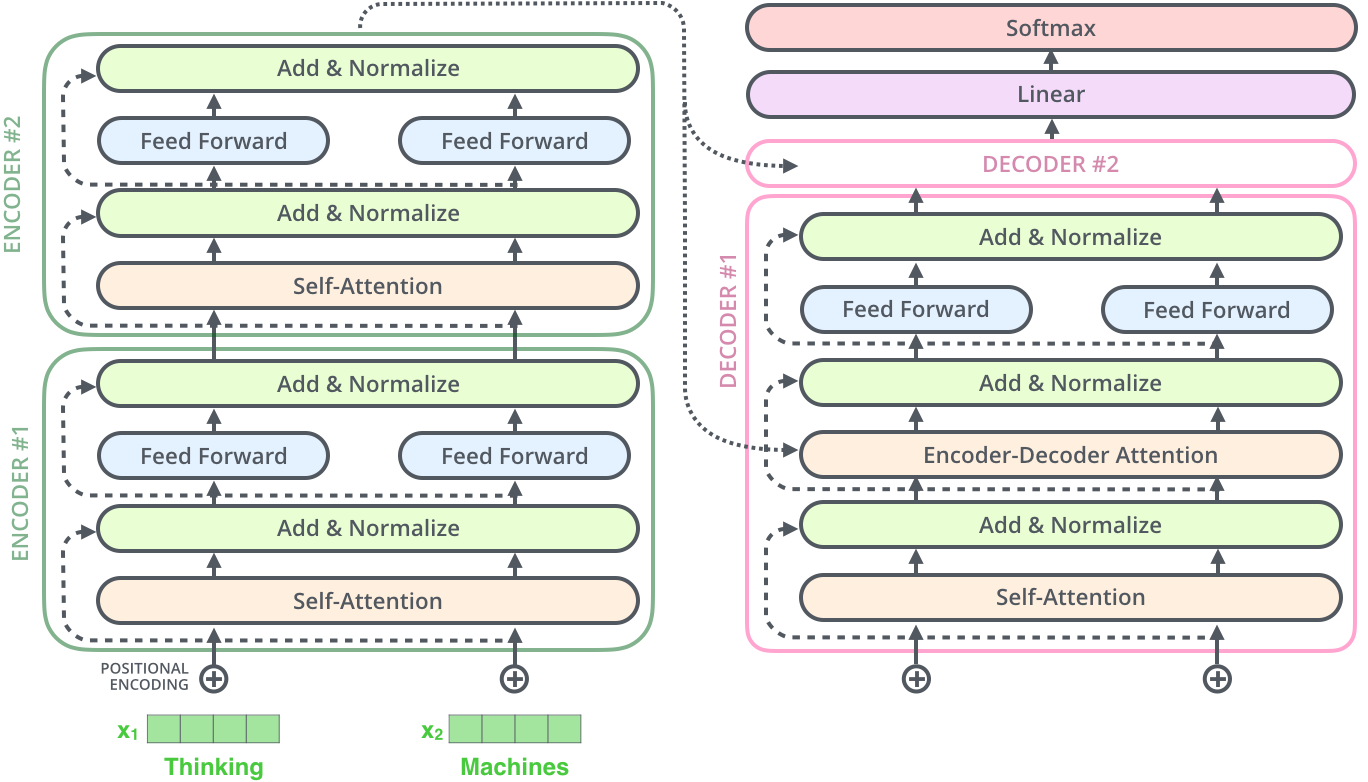
\includegraphics[width=0.9\textwidth]{imgs/encoderDecoderLayersDetailed.png}
    \vspace{-5pt}
    \caption{\scriptsize Transformer: Encoder and Decoder Stack in Detail. \textbf{Encoder layer} contains: (1) Multi-head attention, (2) Position-wise feed forward layer. \textbf{Decoder layer} contains: (1) Masked multi-head attention, (2) Encoder-Decoder attention, (3) Position-wise feed forward layer. From \emph{The Illustrated Transformer}, by Alammar, 2018. \url{https://jalammar.github.io/illustrated-transformer/}. Copyright 2018 by Alammar. }
    %\vspace{-5pt}
    \label{fig:encDecLayersDetailed}
    \end{figure}
    
\end{frame}





% ERASE
% \begin{frame}{Transformer: How Do We Predict a Word?}
%     \footnotesize  
%     
%     Generally ...
%     
%     {\color{MediumVioletRed} \textbf{Encoder Stack $\Rightarrow$ Decoder stack $\Rightarrow$ Linear layer {\scriptsize (logits vector)} $\Rightarrow$ Softmax layer {\scriptsize (probabilities vector)} }}
% 
%     \begin{itemizeSpaced}{7pt}
%     \footnotesize 
%         \item \textbf{Linear Layer} neural network projects Decoder's float vector to larger dimension ``logit vector" (each cell holds a score corresponding to each unique vocabulary word.)
%     
%         \item \textbf{Softmax Layer} then converts the Linear Layer's scores into probabilities via the softmax function. 
%     \end{itemizeSpaced}
% 
%     {\color{MediumVioletRed} \textbf{To find the predicted word: }} the cell with highest probability is chosen $\Rightarrow$ its word is the ``predicted" word. 
% 
%     
% \end{frame}


\section{ELMo (Embeddings from Language Models)}


\begin{frame}{ELMo: Motivation}

    \textbf{Motivation for ELMo: }Remember \textbf{polysemy}? Contextual embeddings create one vector per word type in a context. 
    
    \begin{exampleBlock}{Example}
        If instead models used only word and character embedding, the homonyms ``book" (text) and ``book" (reservation) are assigned the \emph{same vector representation even though these are different words}. 
        
        This vector representation may of course be created using context (as from Word2Vec or GloVe) but contextual meanings get \emph{collapsed into a single representation}.
    \end{exampleBlock}
    
    
\end{frame}



\begin{frame}{ELMo: Structure}

    \begin{itemizeSpaced}{2pt}
        \item \textbf{ELMo} uses bidirectional language model (biLM) to make \emph{deep} word embeddings (derived from all its internal layers)

        \item Higher-level LSTM layers capture contextual meaning (useful for supervised word sense disambiguation (WSD)).
        
        \item Lower layers capture syntax information (useful for part of speech tagging (POS)). 
        
        \item Mixing these signals let ELMo's embeddings select the types of semi-supervision most needed for each end task $\Rightarrow$ ELMo embeddings are thus richer than traditional word vectors. 
        
        \item \textbf{Task-Specific: } ELMo is a task-specific combination of the intermediate layer representations in the biLM (collapses forward and backward hidden states into single embedding for a specific task by weighting the biLM layers): \footnotemark 
        $$
        \textbf{ELMo}_k^{task} = E \Big( R_k; \theta^{task} \Big) = \gamma^{task} \; \sum_{j=0}^L s_j^{task} \; \mathbf{h}_{kj}^{LM}
        $$ 
        
        
    \end{itemizeSpaced}
    
    \footnotetext[10]{ \footnotesize the vector $\mathbf{s}^{task} = \Big\{ s_j^{task} \Big\}$ of softmax-normalized weights and task-dependent scalar parameter $\gamma^{task}$ allow the model for the specific $task$ to scale the entire $\textbf{ELMo}_k^{task}$ vector. The index $k$ corresponds to a $k$-th word, and index $j$ corresponds to the $j$-th layer out of $L$ layers. Here, $h_{kj}^{LM}$ is the output of the $j$-th LSTM for word $k$, and $s_j$ is the weight of $h_{kj}^{LM}$ used to compute the representation for word $k$. }
    
    
\end{frame}



\begin{frame}{ELMo: Example and Key Feature}
    
    
    
    \begin{table}[ht!]
      \centering
      \begin{tabular}{ c }
        
        \begin{minipage}{.9\textwidth}
          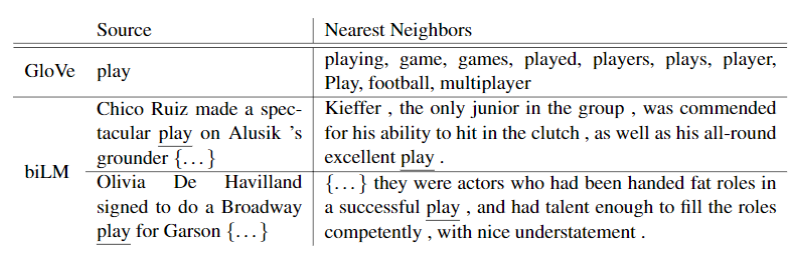
\includegraphics[width=\linewidth]{imgs/table_elmoPlay.png}
        \end{minipage}
        \vspace{-7pt}
      \end{tabular}
      \caption{\linespread{0.3} \footnotesize Nearest neighbors to ``play” using GloVe and the context embeddings from a biLM. From \emph{Table 4 in Deep Contextualized Word Representations}, by Peters et al., 2018. \url{https://arxiv.org/pdf/1802.05365.pdf}. Copyright 2018 by Peters et al.}
      \label{tbl:elmoPlayExample}
      \vspace{-10pt}
    \end{table}
    
    
    \begin{itemizeSpaced}{0pt}
        
        \item \cref{tbl:elmoPlayExample} displays words nearest to polysemous word ``play" found using GloVe vs biLM. 
        
        \item GloVe's neighbors have different parts of speech, like verbs (``played", ``playing"), and nouns (``player", ``game") and only in the sport sense.
        
        
        \item biLM's nearest neighbor sentences from ``play'' CWE show clear difference between \emph{both} the parts of speech \emph{and} word sense of ``play". 
        
        \begin{itemizeSpaced}{0pt}
            \item last row: input sentence has noun / acting sense of ``play" and this is matched in the nearest neighbor sentence
        \end{itemizeSpaced}        
            
    
    \end{itemizeSpaced}
    
    \textbf{ELMo key feature: } learn context using part of speech tagging (POS) and word sense disambiguation (WSD).  
    
\end{frame}
\begin{frame}{}
    \begin{center}
        \large \textbf{BERT (Bidirectional Encoder Representations from Transformers)}
    \end{center}
    \vspace{20pt}
    
    \textbf{Author(s):}
    \begin{itemizeSpaced}{5pt}
    {\color{DimGrey} 
    
        \item Devlin et al. (2019) in \emph{BERT: Pre-training of Deep Bidirectional Transformers for Language Understanding}
        
        \item Clark et al. (2019) in \emph{What Does BERT Look At? An Analysis of BERT's Attention}
        
        \item Wiedemann et al. (2019) in \emph{Does BERT Make Any Sense? Interpretable Word Sense Disambiguation with Contextualized Embeddings}
        
        \item Munikar et al. (2019) in \emph{Fine-Grained Sentiment Classification Using BERT}
        
    }
    \end{itemizeSpaced}
\end{frame}

% -------------------------------------------------




\begin{frame}{\large BERT: Motivation} 
    
    \begin{itemizeSpaced}{7pt}
        \small 
        
        \pinkbox \textbf{Problem with ELMo: } shallowly combines ``independently-trained" biLMs
        
        %\item \textbf{Problem with OpenAI GPT: }unidirectional model $\Rightarrow$ gets no bidirectional context $\Rightarrow$ does poorly on \emph{sentence-level} and \emph{token-level} tasks (question answering (QA))

        
        \pinkbox \textbf{BERT's Solution: } train ``deep bidirectional representations from unlabeled text by jointly conditioning on both left and right context in all layers” (Devlin et al., 2019).
    \end{itemizeSpaced}
    
\end{frame}


\begin{frame}{BERT: Input Embeddings}
    
    \begin{itemizeSpaced}{10pt}
        \footnotesize 
        
        \pinkbox  \textbf{\textit{WordPiece} token embeddings: } \emph{WordPiece} tokenization subdivides words to smaller units 
        
        \vspace{7pt}
        \begin{itemizeSpaced}{7pt}
        
            \footnotesize
            \item to handle rare, unknown words (Weng, 2019) and reduce vocabulary size while increasing amount of data available per word.
            
            \pinkbox \textbf{Example: }if \texttt{"play"} and \texttt{"**ing"} and \texttt{"**ed"} are present in the vocabulary but \texttt{"playing"} and \texttt{"played"} are not, then these can be recognized by their sub-units. 
        \end{itemizeSpaced}
        
        
        \pinkbox \textbf{Segment embeddings: } are arbitrary spans of text (packing sentence parts). 
        NOTE: Transformer-XL respects sentence boundaries. 
        
        \item \textbf{Positional embeddings: } as in ordinary Transformer (to inject word order information). 
    
    \end{itemizeSpaced}
    
\end{frame}




\begin{frame}{BERT Framework: MLM and NSP}

\linespread{0.3} 

BERT does \textbf{pre-training} (on \emph{unlabeled data} using MLM and NSP), and \textbf{fine-tuning} (training on \emph{labeled data} for specific tasks)


{\small \textbf{Masked language model (MLM): }}
    \begin{itemizeSpaced}{5pt}
        \pinkbox \textbf{Motivation:} bidirectional conditioning causes information {\color{MediumVioletRed} leakage} (a word can implicitly ``see itself" letting the model trivially guess the target word in a multi-layered context (Devlin et al., 2019)). 
        
        \item \textbf{Goal: } {\color{MediumVioletRed}randomly masks} some input tokens to predict the original word using context. 
        
        \item \textbf{Effect of MLM: }  {\color{MediumVioletRed}fuses left and right context} to get  {\color{MediumVioletRed}\emph{deep}} bidirectional context (unlike ELMo's  {\color{MediumVioletRed}shallow} left-to-right language model (Devlin et al., 2019)).  
    \end{itemizeSpaced}
    
{\small \textbf{Next Sentence Prediction (NSP):}}
    \begin{itemizeSpaced}{5pt}
        \pinkbox \textbf{Motivation: }  {\color{MediumVioletRed} to capture \emph{sentence-level} information} $\Rightarrow$ to do well in question-answering (QA) and natural language inference (NLI) tasks
        
        
        \item \textbf{Goal: } task that finds if sentence is the next sentence of the other. 
        
    \end{itemizeSpaced}
    
\end{frame}


% \begin{frame}{BERT: General Experimental Results}
% 
%     \begin{itemizeSpaced}{2pt}
%         \item Using a simple accuracy measure, Munikar et al. (2019) found that a pre-trained BERT model fine-tuned for \textbf{sentiment analysis (SA)} task outperformed complex models (RNN, CNNs).
%         
%         \pinkbox This proves \textbf{transfer learning} is possible with BERT's deep contextual bidirectional language model. 
%     \end{itemizeSpaced}
% 
% 
% 
%     \begin{table}[ht!]
%       \centering
%       \vspace{-7pt}
%       
%       \begin{tabular}{ c }
%       
%         \begin{minipage}{.7\textwidth}
%           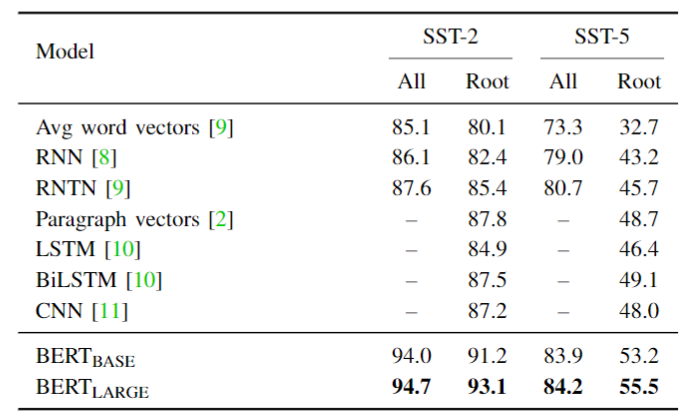
\includegraphics[width=\linewidth]{imgs/table_bert_vsOtherModels.png}
%         \end{minipage}
%         \vspace{-7pt}
%       
%       \end{tabular}
%       
%       \caption{\linespread{0.3} \footnotesize Accuracy (\%) of several models on \textbf{sentiment classification (SC)} SST dataset. BERT has highest accuracy scores. From \emph{Table B.II in Fine-Grained Sentiment Classification Using BERT}, by Munikar et al., 2019. \url{https://arxiv.org/pdf/1910.03474.pdf}. Copyright 2019 by Munikar et al.}
%       \label{tbl:bertExperimentResults}
%       \vspace{-10pt}
%     \end{table}
%     
% \end{frame}



\begin{frame}{Probing BERT: BERT Learns Dependency Syntax}


    \begin{columns}
        
        \begin{column}{0.6\textwidth}
            %\vspace{\topsep}
            \vspace{5pt}
            \begin{center}
            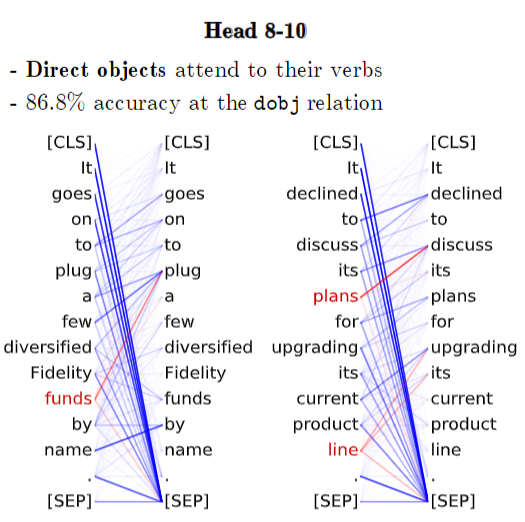
\includegraphics[width=0.8\columnwidth]{imgs/bert_headsDirectObject.png}
            \end{center}
            \vspace{-10pt}
            
            \captionof{figure}{\tiny \linespread{0.2} BERT attention heads capture syntax. In heads 8-10, direct objects are found to attend to their verbs. Line darkness indicates attention strength. Red indicates attention to/from red words, to highlight certain attentional behaviors. From \emph{What Does BERT Look At? An Analysis of BERT's Attention}, by Clark et al., 2019. \url{https://arxiv.org/abs/1906.04341}. } 
            \label{fig:bertHeadDirectObject}
        \end{column}
        
        \begin{column}{0.4\textwidth}
        
            Clark et al. (2019) found ...\newline
            
            \begin{itemizeSpaced}{10pt}
            
                %\scriptsize
                %\item  While BERT's attention heads do not capture syntax dependency structure as a whole....
            
                %\item ... different heads are better at detecting different syntax dependency relationships.
                
                \pinkbox BERT's attention heads detect ``direct objects of verbs, determiners of nouns, objects of prepositions, and objects of possessive pronouns with > $75 \%$ accuracy."
                
                \item Attention heads 8-10 in \cref{fig:bertHeadDirectObject} learn how direct objects attend to their verbs. 
                
                \item BERT learns this using only \textit{self-supervision}. 
            \end{itemizeSpaced}
        \end{column}
    
    \end{columns}


\end{frame}




% 
% \begin{frame}{Probing BERT: BERT's Limitation in Segment Representation}
%     
%     \begin{itemizeSpaced}{10pt}
%         \item BERT does not use separator tokens (\texttt{[SEP]}) to gather segment-level information. 
%         
%         \pinkbox BERT uses \texttt{[SEP]} as ``no-op" or stub operations for attention heads when the head is not needed for a current task. 
%         
%         \item How? Why? Authors investigated in two ways ...
%         
%         \begin{itemizeSpaced}{10pt}
%         
%             \item If this were true, attention heads processing \texttt{[SEP]} should attend broadly over entire segment to make the segment vectors. But in \cref{fig:bertHeadDirectObject}, heads 8-10 show direct objects attend to their verbs, and all other words attend to the \texttt{[SEP]} token. 
%             
%             \item Gradient measures: show much the attention to a token would change BERT's outputs. Attention to \texttt{[SEP]} increases in layers 5-10 (\cref{fig:bertSEPAttention}), WHILE the gradients for attention to \texttt{[SEP]} decrease here (\cref{fig:bertGradient})  $\Rightarrow$ attending to \texttt{[SEP]} does not significantly change BERT's outputs. 
%         \end{itemizeSpaced}
%     \end{itemizeSpaced}
%     
% 
% 
% So, BERT's attention heads attend to \texttt{[SEP]} when they have no other job, not to gather segment-level information. 
% 
% \textbf{Transformer-XL} by design improves this.
% 
% \end{frame}
% 
% 
% 
% 
% 
% \begin{frame}{Probing BERT: BERT's Limitation in Segment Representation}
%     
%     \vspace{10pt}
% 
%     \begin{figure}
%     \centering
%     \begin{minipage}{.47\textwidth}
%       \centering
%       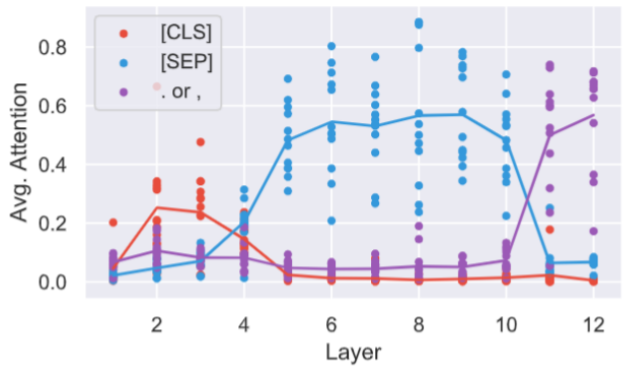
\includegraphics[width=\textwidth]{imgs/bert_attentionSEP_singleimage.png}
%       \vspace{-10pt}
%       \captionof{figure}{\linespread{0.1} BERT's attention heads in layers 6-10 spend more than half the average attention to separator tokens; deep heads attend to punctuation, while middle heads attend to \texttt{[SEP]}, and early heads attend to \texttt{[CLS]}. From \emph{What Does BERT Look At? An Analysis of BERT's Attention}, by Clark et al., 2019. \url{https://arxiv.org/abs/1906.04341}. Copyright 2019 by Clark et al.}
%       \label{fig:bertSEPAttention}
%     \end{minipage} \hspace{2em}%
%     \begin{minipage}{.47\textwidth}
%       \centering
%       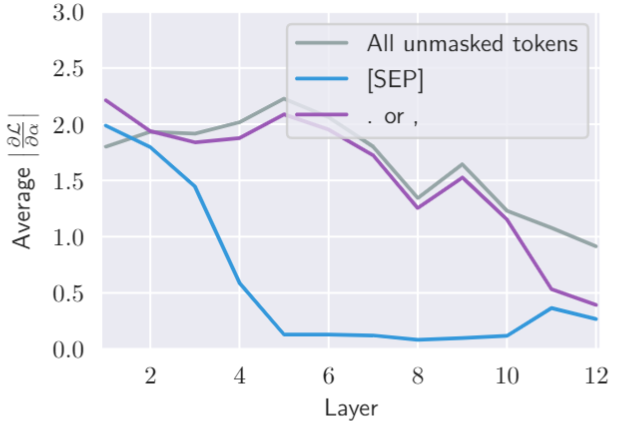
\includegraphics[width=\textwidth]{imgs/bert_attentionheads_gradient.png}
%       \vspace{-15pt}
%       \captionof{figure}{\linespread{0.1} Gradient-based estimates for attention to separator and punctuation tokens. Authors ``compute the magnitude of the gradient of the loss from the masked-language model (MLM) task with respect to each attention weight." From \emph{What Does BERT Look At? An Analysis of BERT's Attention}, by Clark et al., 2019. \url{https://arxiv.org/abs/1906.04341}. Copyright 2019 by Clark et al.}
%       \label{fig:bertGradient}
%     \end{minipage}
%     \end{figure}
% 
%     
% \end{frame}



\begin{frame}{BERT's Attempt at Polysemy}
    
    \vspace{15pt}
    
    \begin{itemizeSpaced}{7pt}
    
        \pinkbox ELMo and BERT were compared on \textbf{word sense disambiguation (WSD)} task $\Rightarrow$ BERT more strongly separates polysemic word senses while ELMo cannot. 
        
        \pinkbox {\color{ForestGreen} BERT did well when} the text had ...
        \vspace{5pt}
        \begin{itemizeSpaced}{7pt}
            \pinkbox \textit{vocabulary overlap}  \texttt{"along the bank of the river"} (input text) and \texttt{"along the bank of the river Greta"} (correct nearest neighbor BERT found). 
            
            \item \textit{semantic overlap} \texttt{"little earthy bank”} (input) and \texttt{"huge bank [of snow]”} (correct nearest neighbor BERT found).
        \end{itemizeSpaced}
        
        \pinkbox {\color{Crimson} BERT struggled when} text had \emph{vocabulary and semantic overlap at the same time}
        
        \begin{itemizeSpaced}{7pt}
        
            %\item \underline{False prediction 1}: BERT predicted \texttt{"land bank" as in a \emph{supply or stock} while the correct sense of \texttt{"land bank" was \emph{financial institution}
            
            \pinkbox \underline{False prediction 1}: for the polysemic word \texttt{"balloon"}, correct word sense was a \emph{verb} but BERT wrongly predicted a \emph{noun} sense.
            
            \item \underline{False prediction 2}: correct sense of \texttt{"watch"} was \emph{to look attentively} while BERT predicted its sense was \emph{to follow with the eyes or the mind; observe}. 
        \end{itemizeSpaced}
        
    \end{itemizeSpaced}
    
\end{frame}


\section{Transformer-XL }


\begin{frame}{Problem with Transformer}
    
    \begin{alertBlock}{Warning: Fixed-Length Context}
        \large 
        
        Transformers have \textbf{\alert{fixed-length context}} (limited context dependency), meaning the largest dependency distance between characters is limited by input length. 
        
        Also, natural semantic boundaries formed by sentences are \textit{not} respected. 
        
        \begin{addmargin}{3em}{}
        \begin{itemizeSpaced}{2pt}
            \arrowitem Transformers lose contextual information 
            
            \arrowitem Transformers forget words from a few sentences ago (Dai et al., 2019) 
            
            \arrowitem long-term memory problem.
            
            \arrowitem \textbf{Context-Fragmentation Problem}
        \end{itemizeSpaced}
        \end{addmargin} 
        
    \end{alertBlock}
    

\end{frame}
    
    
\begin{frame}{Problem with Transformer: Fixed-Length Context Illustrated}
    

    \begin{figure}[h]
    \vspace{-5pt}
    \centering
    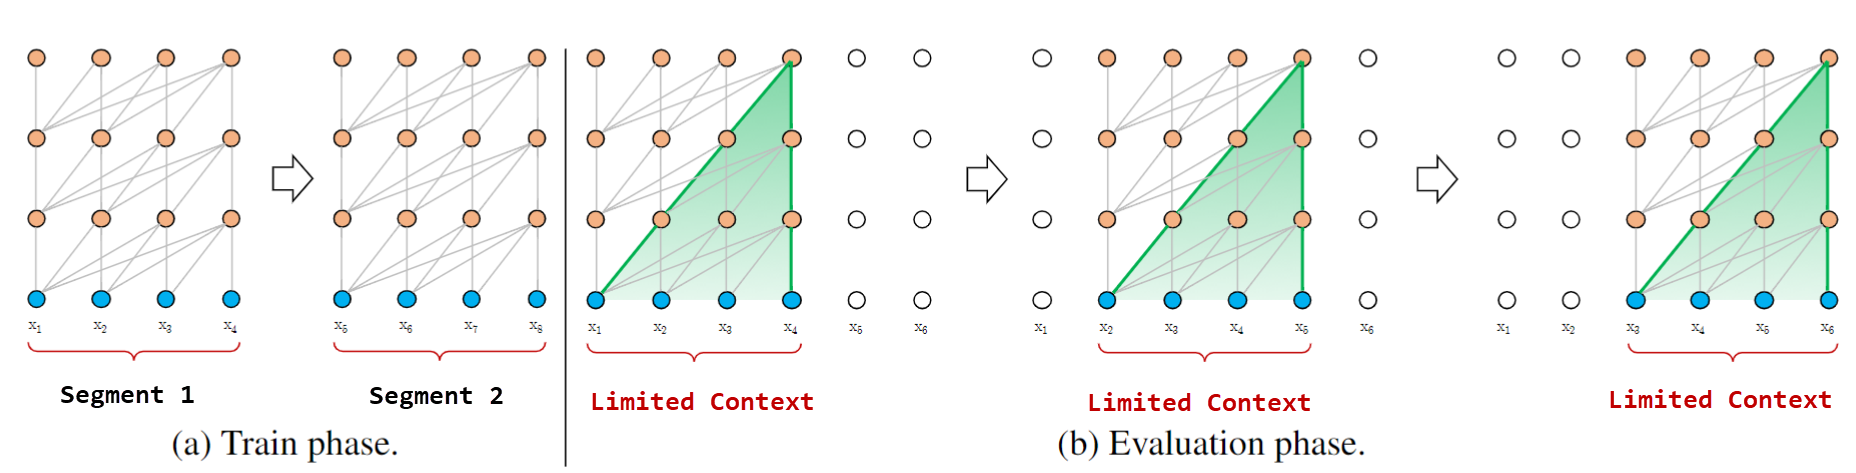
\includegraphics[width=0.99\textwidth]{imgs/transXL_vanillaSegmentation.png}
    %\vspace{-5pt}
    \caption{\small Vanilla Transformer with segment embedding length $ = 4$. Training the model in fixed-length segments while disregarding natural sentence boundaries results in the \emph{context fragmentation problem}: during each evaluation step, the Transformer consumes a segment embedding and makes a prediction at the last position. Then at the next step, the segment is shifted right by one position only, and the new segment must be processed from scratch, so there is no context dependency for first tokens of each segment and between segments. From \emph{Transformer-XL: Attentive Language Models Beyond a Fixed-Length Context}, by Dai et al., 2019. \url{https://arxiv.org/pdf/1901.02860.pdf}. Copyright 2019 by Dai et al.}
    \vspace{-5pt}
    \label{fig:transXL_VanillaSegment}
    \end{figure}
    
\end{frame}



\begin{frame}{Motivation for Transformer-XL}

    \large 
    \linespread{0.5}
    
    \begin{itemizeSpaced}{15pt}
        \item \textbf{Transformer-XL} (extra long) learns longer dependencies without ``disrupting temporal coherence"  (Dai et al., 2019). 
        
        \item Doesn't chop sentences into arbitrary \textbf{fixed lengths}!
        
        \pinkbox Transformer-XL \emph{respects natural language boundaries} like sentences and paragraphs, helping it gain richer context over sentences, paragraphs, and even longer texts like documents. 
        
        \pinkbox Transformer-XL is composed of \textbf{segment-level recurrence mechanism} and \textbf{relative positional encoding} method (to fix \textbf{context fragmentation} and represent longer-spanning dependencies)
    \end{itemizeSpaced}
    
\end{frame}


\begin{frame}{Transformer-XL: Segment-Level Recurrence Mechanism}

    \linespread{0.3}
    
    When a segment is being processed, each hidden layer receives two inputs: 
    
    \begin{itemizeSpaced}{10pt}
        \item the previous hidden layer outputs of the \emph{current segment} (like vanilla transformer, visible as gray arrows in \cref{fig:transXL_extendedContext})
        
        \item the previous hidden layer outputs of the \emph{previous segment} (green arrows in \cref{fig:transXL_extendedContext}).
    \end{itemizeSpaced}
    
    
    
    \begin{figure}[h]
    \vspace{-5pt}
    \centering
    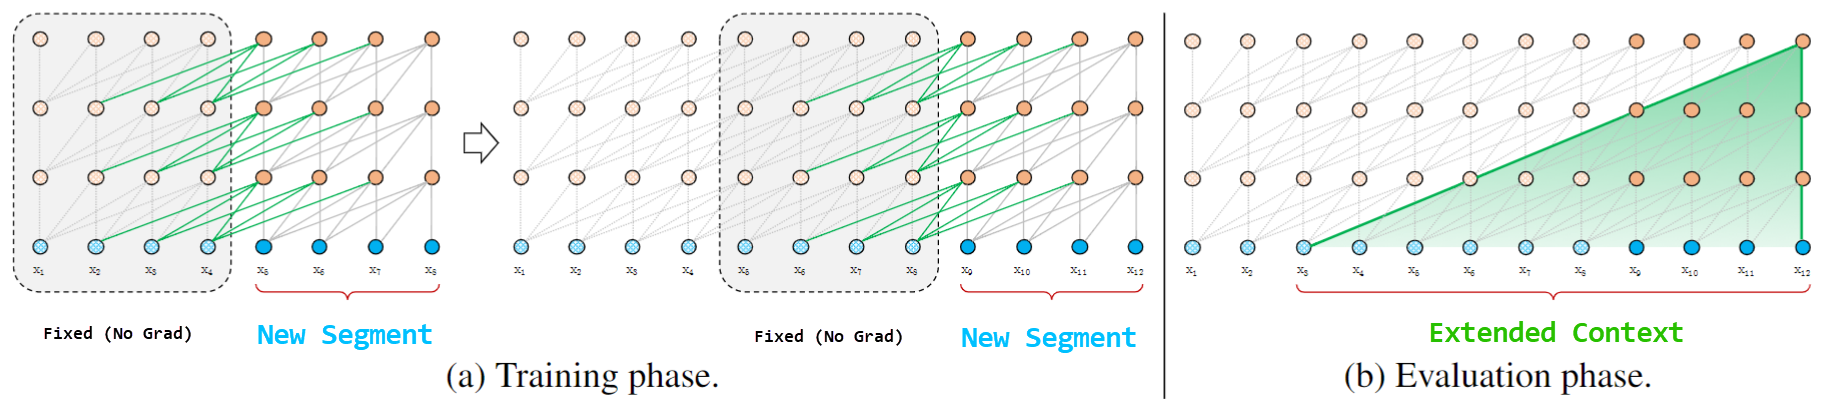
\includegraphics[width=0.99\textwidth]{imgs/transXL_extendedcontext.png}
    %\vspace{-5pt}
    \caption{\small Segment level recurrence mechanism at work: the hidden state for previous segment is \emph{fixed} and \emph{stored} to later be reused as extended context while new segment is processed. Like in Transformer, gradient updates (training) still occurs within a segment, but extended context includes historical information. From \emph{Transformer-XL: Attentive Language Models Beyond a Fixed-Length Context}, by Dai et al., 2019. \url{https://arxiv.org/pdf/1901.02860.pdf}. Copyright 2019 by Dai et al.}
    %\vspace{-5pt}
    \label{fig:transXL_extendedContext}
    \end{figure}
    
\end{frame}



\begin{frame}{Transformer-XL: Relative Positional Encoding}
    \normalsize\linespread{1.0}

    \begin{alertBlock}{Problem when using Segment-Level Recurrence}
    
        How can positional word order be kept coherent when reusing hidden states?
        
        Standard Transformer uses positional encodings (use absolute distance between tokens) .
    
        \begin{addmargin}{3em}{} % 3em left, NOTHING right
        \begin{itemizeSpaced}{5pt}
            \largearrowitem Applying to Transformer-XL caused consecutive word embedding sequences to be associated with the same positional encoding.
            
            \largearrowitem Transformer-XL can't distinguish the difference in positions of consecutive input tokens.
            
            \largearrowitem Tokens from different segments had the same positional encodings, defeating the purpose.
        \end{itemizeSpaced}
        \end{addmargin} 
        
        
    \end{alertBlock} 
    
    {\large \textbf{Solution: Relative Positional Encodings}}
    
    \begin{itemizeSpaced}{0pt}
        \item uses \emph{relative} distance between tokens 
        
        \item injects this into \emph{each} attention score of each layer (rather than before first layer).
    \end{itemizeSpaced}

    
\end{frame}



\begin{frame}{Transformer-XL: Experimental Results}
    
    Ablation study: Isolating effects of \textbf{segment-level recurrence mechanism} with different encoding schemes (Shaw (2018) uses relative, and Vaswani / Al-Rfou use absolute).
        
    \begin{itemize}
        \item \textbf{KEY: }best results obtained using \emph{both}  segment-level recurrence and relative positional encoding.
    \end{itemize}
        
    
    \begin{figure}[h]
    \vspace{-5pt}
    \centering
    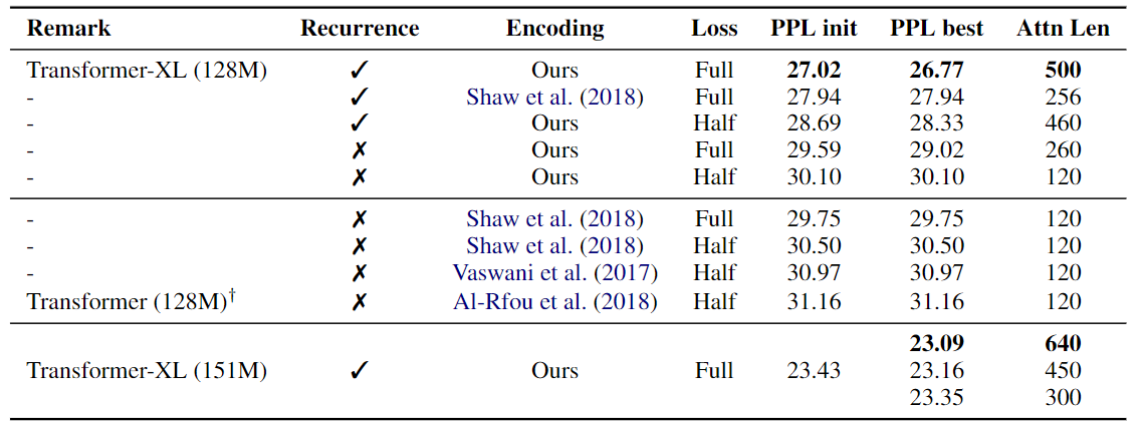
\includegraphics[width=0.99\textwidth]{imgs/table_transXL_ablationREC.png}
    \vspace{-5pt}
    \captionof{table}{\linespread{0.3}\footnotesize Ablation study for segment-level recurrence on the WikiText-103 data set. \textbf{PPL best} (model output) means perplexity score obtained using an optimal backpropagation training time length. \textbf{Attn Len} (model input) is the shortest possible attention length during evaluation to achieve the corresponding PPL best. From \emph{Transformer-XL: Attentive Language Models Beyond a Fixed-Length Context}, by Dai et al., 2019. \url{https://arxiv.org/pdf/1901.02860.pdf}. Copyright 2019 by Dai et al.}
    \vspace{-5pt}
    \label{tbl:transXL_ablationRECURR}
    \end{figure}

\end{frame}


\section{XLNet}


\begin{frame}{XLNet: Problems with BERT}

\begin{itemizeSpaced}{7pt}
    \pinkbox An \textbf{autoregressive language model (AR)} autoregressively estimates the probability distribution of a text sequence by factorizing a likelihood using tokens \emph{before} a timestep, or tokens \emph{after} a timestep. A neural network is trained to model either the forward or backward distribution $\Rightarrow$ cannot model bidirectional context. 
    
    \item An \textbf{autoencoding language model (AE)} like BERT is like a masked language model. It masks tokens, predicts them and does not estimate densities like AR $\Rightarrow$ can learn bidirectional contexts. 
    
    \pinkbox \textbf{BERT's problems: }
    \begin{itemizeSpaced}{7pt}
        
        \item \textbf{False Independence Assumption: } BERT factorizes its log likelihood probability assuming all masked tokens are rebuilt independently of each other (so BERT ignores long-term dependencies within texts)
        
        \item \textbf{Data Corruption: }Masked tokens do not appear in real data during fine-tuning, so since BERT uses them in pre-training, a discrepancy arises between these two steps. 
    \end{itemizeSpaced}
    
    
\end{itemizeSpaced}


    
\end{frame}


\begin{frame}{XLNet: Example of BERT's False Independence Assumption}
    
\begin{exampleBlock}{Example: BERT predicting tokens independently}
``I went to the \texttt{[MASK]} \texttt{[MASK]} and saw the \texttt{[MASK]} \texttt{[MASK]} \texttt{[MASK]}." 

Two ways to fill this are: 

``I went to \emph{New York} and saw the \textit{Empire State building}," or

``I went to \emph{San Francisco} and saw the \emph{Golden Gate bridge}."

But BERT might incorrectly predict something like: ``I went to \emph{San Francisco} and saw the \emph{Empire State building}." 

Independence assumption + predicting masked tokens simultaneously $\Rightarrow$ BERT fails to learn their interlocking dependencies $\Rightarrow$ weakens the ``learning signal" (Kurita, 2019b). 
\end{exampleBlock}

\end{frame}


\begin{frame}{XLNet: Motivation}

\large 

To keep benefits of both autoencoding and autoregressive modeling while avoiding their issues...

\begin{enumerateSpaced}{7pt}
    \item XLNet adopts an AR model so that probability of a token can be factored via product rule, eliminating BERT's false independence assumption. 
    
    \item XLNet uses \textbf{permutation language model} to capture bidirectional context AND \textbf{two-stream attention} to adapt its Transformer to create target-aware predictions. 
\end{enumerateSpaced}
    
\end{frame}



\begin{frame}{XLNet; Permutation Language Model}
    
    
    \textbf{Created so that: } a model can be trained to use \textbf{bidirectional context} while avoiding masking and its resulting problem of independent predictions.

    \vspace{20pt}
    
    \begin{definitionBlock}{Definition: Permutation Language Model}
    Like language models, a \textbf{permutation language model} predicts unidirectionally. 
    
    But instead of predicting in order, the model predicts tokens in a random order. 
    
    Is forced to accumulate bidirectional context by finding dependencies between \emph{all} possible input combinations. 
    
    (NOTE: only permutes factorization order, not order of word inputs)
    \end{definitionBlock}
    
\end{frame}


\begin{frame}{XLNet: Target-Aware Predictions}
    \begin{itemizeSpaced}{5pt}
        \item {\color{Crimson} \textbf{Problem: }} Trying to merge permutation language model and Transformer made XLNet’s target predictions blind to the permutation positions generated by the permutation language model.

        \item Fault is due to Transformer: while predicting a token at a position, the model masks the token’s embedding AND also its \emph{positional} encoding $\Rightarrow$ Transformer remains blind about the position of the target it should be predicting $\Rightarrow$  sentence cannot be accurately represented (since positions like the beginning of a sentence have different distributions from other positions in the sentence.)
        
        \item {\color{ForestGreen} \textbf{Solution: Target-awareness: }} authors adapted the predictive distribution to take the target position as an argument $\Rightarrow$ now can create target-aware embeddings. 
        
        \item {\color{Crimson} \textbf{Another problem}: }aforementioned problem with Transformer creates a contradiction: (1) to predict the content token $x_{z_t}$, only the position is needed, not the content $x_{z_t}$, and (2) to predict all other tokens $x_{z_j}$, the content token is  needed. 
        
        \item {\color{ForestGreen} \textbf{Two-Stream Attention: }}uses two sets of hidden states (content stream and query stream) to create an overall hidden state. 
        
        {\linespread{0.3}
        \begin{itemizeSpaced}{5pt}
            \item \textbf{Content-Stream Attention: } encodes \emph{context} like an ordinary Transformer, along with the \emph{content} (prediction) token $x_{z_t}$
            
            \item \textbf{Query-Stream Attention: }encodes \emph{context} with target token's \emph{position} but NOT content (prediction) token $x_{z_t}$ (to evade the contradiction). 
        \end{itemizeSpaced} }
        
    \end{itemizeSpaced}
\end{frame}


\begin{frame}{XLNet: Relative Segment Encodings}
    \normalsize
    \begin{itemizeSpaced}{10pt}
        \item XLNet adopts Transformer-XL's idea of relative encodings. 
        
        \item BERT's segment embeddings distinguish words belonging to different segments. 
        
        \pinkbox XLNet's segment embeddings encode if two words are \emph{within the same segment} rather than \emph{which specific segments the words are from} $\Rightarrow$ can apply XLNet to tasks that intake arbitrarily many sequences. 
    \end{itemizeSpaced}
    
\end{frame}


\begin{frame}{XLNet: Conceptual Difference with BERT}

Illustrating the conceptual difference between XLNet and BERT from a model training standpoint: 

    \begin{exampleBlock}{Example: Conceptual Difference between XLNet and BERT}
    

    Take the list of words $\Big[ \texttt{New}, \texttt{York}, \texttt{is}, \texttt{a}, \texttt{city} \Big]$. 
    
    Prediction tokens: $\Big[ \texttt{New}, \texttt{York} \Big]$ 
    
    XLNet and BERT must maximize the log-likelihood: $\text{log} \; P(\texttt{New York} \; | \; \texttt{is a city})$. 
    
    Assumption: XLNet uses the factorization order $\Big[ \texttt{is}, \texttt{a}, \texttt{city}, \texttt{New}, \texttt{York} \Big]$
    
    Then each of their loss functions are: 
    
    \begin{equation}
    \begin{array}{ll}
    \mathcal{J}_\text{BERT} = \text{log} \; P \Big( \texttt{New} \; | \; \texttt{is a city} \Big) \; + \; \text{log} \; P \Big( \texttt{York} \; | \; \texttt{is a city} \Big) \\
    \mathcal{J}_\text{XLNet} = \text{log} \; P \Big( \texttt{New} \; | \; \texttt{is a city} \Big) \; + \; \text{log} \; P \Big( \texttt{York} \; | \; {\color{cyan} \texttt{New}}, \texttt{is a city} \Big) 
    \end{array}
    \end{equation}
    
    Result: XLNet learns a stronger dependency than BERT between the pairs \texttt{New} and \texttt{York} (Dai et al., 2019). 
    
    \end{exampleBlock}
    
\end{frame}


\begin{frame}{}
    \begin{center}
        \large \textbf{ERNIE 1.0: Enhanced Representations through Knowledge Integration}
    \end{center}
    \vspace{20pt}
    
    \textbf{Author(s):}
    \begin{itemizeSpaced}{5pt}
    {\color{DimGrey} 
    
        \item Sun et al. (2019a) in \emph{ERNIE: Enhanced Representations Through Knowledge Integration}
        
    }
    \end{itemizeSpaced}
\end{frame}

% -------------------------------------------------




\begin{frame}{ERNIE: Motivations}

    \vspace{10pt}
    
    \begin{itemizeSpaced}{2pt}
        \pinkbox Previous models (Word2Vec, GloVe, BERT) make embeddings via context and co-occurrence $\Rightarrow$ fail to use prior knowledge (tucked away in sentence ordering and proximity) to capture relationships between entities. 
    \end{itemizeSpaced}

    
    \vspace{-5pt}
    \begin{exampleBlock}{Example: ERNIE's Entity Capturing Skills}
        
        Consider the following training sentence: \newline 
        
        {\footnotesize \textit{``Harry Potter is a series of fantasy novels written by J. K. Rowling."}}\newline 
        
        Using co-occurring words ``J.", ``K.", and ``Rowling", BERT is limited to predicting the token ``K." but utterly fails at recognizing the whole entity \emph{J. K. Rowling}. \newline 
        
        A model could use simple co-occurrence counts to predict \emph{Harry Potter} ... but not via the \emph{\alert{relationship between novel and  writer}}. 
    \end{exampleBlock}


    \vspace{-5pt}
    \begin{itemizeSpaced}{2pt} 
        
        \pinkbox {\color{ForestGreen} \footnotesize \textbf{ERNIE to the rescue! }} ERNIE can extrapolate the relationship between the \emph{Harry Potter} entity and \emph{J. K. Rowling} entity using implicit knowledge of words and entities $\Rightarrow$ can predict Harry Potter is a series written by J. K. Rowling (Sun et al., 2019a). 
    
    \end{itemizeSpaced}
    
\end{frame}


\begin{frame}{ERNIE: Phrase and Entity-Level Masking}

    \vspace{10pt}
    
    \begin{itemizeSpaced}{5pt}
        \item ERNIE uses a Transformer Encoder coupled with \textbf{entity-level masking} and \textbf{phrase-level masking} (to encode prior knowledge in {\color{DodgerBlue} conceptual units} like phrases and entities) $\Rightarrow$ learns longer semantic dependencies, has better generalization, adaptability. 
        
        \item \textbf{Phrase-level masking: } A phrase is a ``small group of words or characters acting as a {\color{DodgerBlue} conceptual unit}" (Sun et al., 2019a). ERNIE chunks sentences to find phrase boundaries, then masks and predicts them. 
        
        \item \textbf{Entity-level masking: } name entities contain ``persons, locations, organizations, products." Often include conceptual information. ERNIE parses the entities from a sentence, masks them, then predicts all slots within entities, as shown in \cref{fig:ernie_maskingTypes}.
        
    \end{itemizeSpaced}
    
    
    
    \begin{figure}[h]
    \vspace{-5pt}
    \centering
    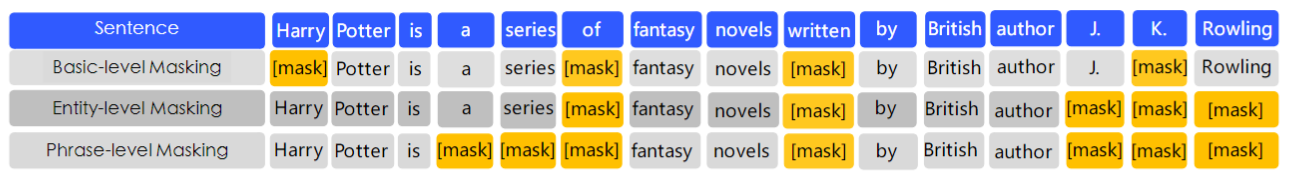
\includegraphics[width=0.99\textwidth]{imgs/ernie_maskingtypes.png}
    \vspace{-5pt}
    \captionof{figure}{\linespread{0.3}\scriptsize ERNIE uses basic masking to get word representations, followed by phrase-level and entity-level masking. From \emph{ERNIE: Enhanced Representation Through Knowledge Integration}, by Sun et al., 2019a. \url{https://arxiv.org/pdf/1904.09223.pdf}. Copyright 2019 by Sun et al.}
    \vspace{-5pt}
    \label{fig:ernie_maskingTypes}
    \end{figure}
    
    
\end{frame}



\begin{frame}{ERNIE: Knowledge Learning To Fill-In-Blanks on Named Entities}

\vspace{10pt}

\begin{table}[htbp]
    \scriptsize 
    \centering \linespread{0.3}
    \setlength{\tabcolsep}{4pt} % Default value: 6pt
    \renewcommand{\arraystretch}{3} % Default value: 1
    
    \begin{tableFont}
    \begin{tabu} to \textwidth {| X[0.4] | X[6] | X | X | X |}
        
    
        \hline
      
        %\rowcolor{MyLavender} 
        \centering \textbf{Case}
        & \centering \textbf{Text} 
        & \centering \textbf{ERNIE}
        & \centering\textbf{BERT} 
        & \centering \textbf{Answer} \\ 
        
        \hline
        
        
        $1$
        &
        ``In September 2006, $\_\_\_$ married Cecilia Cheung. They had two sons, the older one is Zhenxuan Xie and the younger one is Zhennan Xie." \newline
        & 
        Tingfeng Xie
        & 
        Zhenxuan Xie
        & 
        {\color{Green} \textbf{Tingfeng Xie}} \\ 
        
        \hline 
        
        
        
        $4$
        &
        ``Australia is a highly developed capitalist country with $\_\_\_$ as its capital. As the most developed country in the Southern Hemisphere, the $12$th largest economy in the world and the fourth largest exporter of agricultural products in the world, it is also the world's largest exporter of various minerals."   \newline 
        & 
        Melbourne
        & 
        (Not a city name)
        & 
        {\color{Green} \textbf{Canberra}} \\ 
        
        \hline 
        
        $6$
        &
        ``Relativity is a theory about space-time and gravity, which was founded by $\_\_\_$."   
        & 
        Einstein
        & 
        (Not a word in Chinese)
        & 
        {\color{Green} \textbf{Einstein}} \\ 
        
        
        \hline 
    \end{tabu}
    
    \end{tableFont}
    
    \vspace{-5pt}
    
    \captionof{table}{\linespread{0.2}\scriptsize Comparing ERNIE to BERT on Cloze Chinese Task. From \emph{Figure 4 in ERNIE: Enhanced Representation Through Knowledge Integration}, by Sun et al., 2019a. Copyright 2019 by Sun et al.}
    
    \label{tbl:ernie_vs_bert_knowledgeLearningTask}
\end{table}
\vspace{-10pt}



\vspace{-10pt}
\begin{itemizeSpaced}{0pt}
    \linespread{0.1}
    \item Case 1: ERNIE predicts the correct father name entity based on prior knowledge in the article while BERT simply memorizes a son's name, completely ignoring any relationship between mother and son. 
    
    \item Case 4, 6: BERT fills the slots with characters related to the sentences but not with the semantic concept. 
    
    \item Case 4: ERNIE predicts the wrong city name, though it still understands the semantic type.
\end{itemizeSpaced}

ERNIE's contextual knowledge understanding is far superior to BERT's!
    
\end{frame}



\begin{frame}{Question and Answer Session}
    
    \large \centering \textbf{Questions? }
\end{frame}


\begin{frame}{References}


\vspace{10pt}
\begin{enumerateSpaced}{4pt}
    \scriptsize
    
    \item Smith, and A., N. (2019, February 19). Contextual Word Representations: A Contextual Introduction. Retrieved from \url{https://arxiv.org/abs/1902.06006}

    \item Melamud, O., Goldberger, et al. (2016). context2vec: Learning Generic Context Embedding with Bidirectional LSTM. \emph{Proceedings of The 20th SIGNLL Conference on Computational Natural Language Learning}. doi: 10.18653/v1/k16-1006
    
    \item Devlin, Jacob, et al. (2019, May 24). BERT: Pre-training of Deep Bidirectional Transformers for Language Understanding. Retrieved from \url{https://arxiv.org/abs/1810.04805}
    
    \item Wiedemann, Gregor, et al. (2019, September 23). Does BERT Make Any Sense? Interpretable Word Sense Disambiguation with Contextualized Embeddings. Retrieved from \url{https://arxiv.org/abs/1909.10430v1}
    
    \item Munikar, M., et al. (2019). Fine-grained Sentiment Classification using BERT. 2019 \emph{Artificial Intelligence for Transforming Business and Society (AITB)}. doi: 10.1109/aitb48515.2019.8947435
    
    \item Clark, K., et al. (2019). What Does BERT Look at? An Analysis of BERT’s Attention. \emph{Proceedings of the 2019 ACL Workshop BlackboxNLP: Analyzing and Interpreting Neural Networks for NLP}. doi: 10.18653/v1/w19-4828
    
    \item Ethayarajh, K. (2019). How Contextual are Contextualized Word Representations? Comparing the Geometry of BERT, ELMo, and GPT-2 Embeddings. \emph{Proceedings of the 2019 Conference on Empirical Methods in Natural Language Processing and the 9th International Joint Conference on Natural Language Processing (EMNLP-IJCNLP).} doi: 10.18653/v1/d19-1006

\end{enumerateSpaced}
    
\end{frame}



\begin{frame}{}

\begin{enumerateSpaced}{5pt}
    \scriptsize
    \setcounter{enumi}{7}
    

    \item Batista, D. (n.d.). Language Models and Contextualised Word Embeddings. Retrieved from \url{http://www.davidsbatista.net/blog/2018/12/06/Word_Embeddings/}
    
    \item Neelakantan, A., et al. (2014). Efficient Non-parametric Estimation of Multiple Embeddings per Word in Vector Space. \emph{Proceedings of the 2014 Conference on Empirical Methods in Natural Language Processing (EMNLP).} doi: 10.3115/v1/d14-1113
    
    \item Antonio, M. (2019, September 5). Word Embedding, Character Embedding and Contextual Embedding in BiDAF - an Illustrated Guide. Retrieved from \url{https://towardsdatascience.com/the-definitive-guide-to-bidaf-part-2-word-embedding-character-embedding-and-contextual-c151fc4f05bb}
    
    \item Mikolov, T., Sutskever, I., et al. (2013a, October 16). Distributed Representations of Words and Phrases and their Compositionality. Retrieved from \url{https://arxiv.org/pdf/1310.4546.pdf}
    
    \item Mikolov, Tomas, et al. (2013b, September 7). Efficient Estimation of Word Representations in Vector Space. Retrieved from \url{https://arxiv.org/abs/1301.3781}
    
    \item Weng, L. (2017, October 15). Learning Word Embedding. Retrieved from \url{https://lilianweng.github.io/lil-log/2017/10/15/learning-word-embedding.html}


    \item Pennington, J., Socher, R., and Manning, C. (2014). Glove: Global Vectors for Word Representation.\emph{edings of the 2014 Conference on Empirical Methods in Natural Language Processing (EMNLP)}.doi: 10.3115/v1/d14-1162
    
\end{enumerateSpaced}
    
\end{frame}




\begin{frame}{}
    
    
    \begin{enumerateSpaced}{5pt}
    
        \scriptsize
        \setcounter{enumi}{14}
        
        
        \item Kurita, K. (2018a, May 4). Paper Dissected: "Glove: Global Vectors for Word Representation" Explained. Retrieved from \url{http://mlexplained.com/2018/04/29/paper-dissected-glove-global-vectors-for-word-representation-explained/}
        
        \item Sutskever, I., et al. (2014, December 14). Sequence to Sequence Learning with Neural Networks. Retrieved from \url{https://arxiv.org/abs/1409.3215}
        
        \item Vaswani, Ashish, et al. (2017, December 6). Attention Is All You Need. Retrieved from \url{https://arxiv.org/abs/1706.03762}
        
        \item G, R. (2019, March 18). Transformer Explained - Part 1. Retrieved from \url{https://graviraja.github.io/transformer/}
        
        \item Ta-Chun. (2018, October 3). Seq2seq pay Attention to Self Attention: Part 1. Retrieved from \url{https://medium.com/@bgg/seq2seq-pay-attention-to-self-attention-part-1-d332e85e9aad}
        
        \item Alammar, Jay. “Visualizing A Neural Machine Translation Model (Mechanics of Seq2seq Models With Attention).” \emph{Visualizing A Neural Machine Translation Model (Mechanics of Seq2seq Models With Attention) – Jay Alammar – Visualizing Machine Learning One Concept at a Time}, 2018a, \url{jalammar.github.io/visualizing-neural-machine-translation-mechanics-of-seq2seq-models-with-attention/}.
        
        \item Alammar, J. (2018b, June 27). The Illustrated Transformer. Retrieved from \url{http://jalammar.github.io/illustrated-transformer/}
    
    \end{enumerateSpaced}
    
    
\end{frame}



\begin{frame}{}

    \begin{enumerateSpaced}{3pt}
    
        \scriptsize
        \setcounter{enumi}{21}
        
    
        \item Peters, et al. “Deep Contextualized Word Representations.” \emph{ArXiv.org}, (22 Mar. 2018), \url{arxiv.org/abs/1802.05365}.
        
        \item Dai, Zihang, et al. “Transformer-XL: Attentive Language Models beyond a Fixed-Length Context.” \emph{Proceedings of the 57th Annual Meeting of the Association for Computational Linguistics}, (2019), \url{https://arxiv.org/pdf/1901.02860.pdf}.
        
        \item Yang, Z, et al. "XLNet: Generalized Autoregressive Pretraining for Language Understanding." \emph{Proceedings of the 57th Annual Meeting of the Association for Computational Linguistics}, (2020), \url{https://arxiv.org/pdf/1906.08237.pdf}.
        
        \item Kurita, Keita. “Paper Dissected: ‘XLNet: Generalized Autoregressive Pretraining for Language Understanding’ Explained.” \emph{Machine Learning Explained}, (7 July 2019b), \url{mlexplained.com/2019/06/30/paper-dissected-xlnet-generalized-autoregressive-pretraining-for-language-understanding-explained/}.
        
        
        \item Sun, Y, et al. "ERNIE: Enhanced Representations Through Knowledge Integration." \emph{Proceedings of the 57th Annual Meeting of the Association for Computational Linguistics}, (2019a), \url{https://arxiv.org/pdf/1904.09223.pdf}.
        
        \item Sun, Y, et al. "ERNIE 2.0: A Continual Pre-Training Framework for Language Understanding." \emph{Proceedings of the 57th Annual Meeting of the Association for Computational Linguistics}, (2019b), \url{https://arxiv.org/pdf/1907.12412.pdf}.
        
        
        
    \end{enumerateSpaced}
    
\end{frame}




\end{document}






%%% Local Variables: 
%%% mode: latex
%%% TeX-PDF-mode: t 
%%% TeX-master: t
%%% End: 